\pdfoutput=1
\documentclass[journal, 10pt]{IEEEtran}
\IEEEoverridecommandlockouts
%\documentclass[11pt,draftcls,onecolumn]{IEEEtran}
%\usepackage{geometry}   
%\usepackage[margin=1in]{geometry}             % See geometry.pdf to learn the layout options. There are lots.
%\geometry{letterpaper}                   % ... or a4paper or a5paper or ... 
%\geometry{landscape}                % Activate for for rotated page geometry
%\usepackage[parfill]{parskip}    % Activate to begin paragraphs with an empty line rather than an indent
\usepackage{graphicx}
\usepackage{amssymb}
\usepackage{amsmath}
\usepackage{amsthm}
\usepackage{amsfonts}
\usepackage{hyperref,algorithm}
\usepackage{algpseudocode}
\usepackage{mathtools}
\usepackage{epstopdf}
\usepackage{dblfloatfix}
\usepackage{color}
\usepackage{array}
\usepackage{arydshln}
\usepackage{multirow}
\usepackage{booktabs}
\usepackage{balance}
\usepackage{setspace}
\DeclareGraphicsRule{.tif}{png}{.png}{`convert #1 `dirname #1`/`basename #1 .tif`.png}
\newtheorem{theorem}{\textbf{Theorem}}
\newtheorem{definition}{\textbf{Definition}}
\newtheorem{problem}{\textbf{Problem}}
\newtheorem{example}{\textbf{Example}}
\newtheorem{remark}{\textbf{Remark}}
\newtheorem{lemma}{\textbf{Lemma}}
\newtheorem{corollary}{\textbf{Corollary}}
\newtheorem{proposition}{\textbf{Proposition}}
\newcommand{\transpose}{{\!\scriptscriptstyle\mathrm T}}
\newcommand{\norm}[1]{\lVert#1\rVert}
\newcommand{\R}{\mathbb{R}}
\renewcommand{\l}{\ell}
\newcommand{\Identity}{1\!\!1}
\newcommand{\G}{{\mathcal{G}}}
\newcommand{\E}{{\mathcal{E}}}
\newcommand{\W}{{\mathcal{W}}}
\newcommand{\V}{{\mathcal{V}}}
\newcommand\ip[2]{\langle #1, #2\rangle}
\usepackage{array}
\newcolumntype{L}[1]{>{\raggedright\let\newline\\\arraybackslash\hspace{0pt}}m{#1}}
\newcolumntype{C}[1]{>{\centering\let\newline\\\arraybackslash\hspace{0pt}}m{#1}}
\newcolumntype{R}[1]{>{\raggedleft\let\newline\\\arraybackslash\hspace{0pt}}m{#1}}
\renewcommand{\L}{\boldsymbol{\mathcal{L}}}
 \DeclareMathOperator*{\argmax}{argmax}
 \DeclareMathOperator*{\argmin}{argmin}
\newcommand{\Expectation}{I\!\!E} %expectation
\renewcommand{\IEEEbibitemsep}{0pt plus 0.5pt}
\newcommand{\change}[1]{{\color{blue} {#1} }}
\makeatletter
\IEEEtriggercmd{\reset@font\normalfont\fontsize{7.5pt}{8.0pt}\selectfont}
\makeatother
\IEEEtriggeratref{1}

\begin{document}

\title{
A Scalable $M$-Channel Critically Sampled Filter Bank for Graph Signals 
}
\author{\IEEEauthorblockN{Yan Jin, Shuni Li, and David I Shuman}
%\thanks{Copyright (c) 2015 IEEE. Personal use of this material is permitted. However, permission to use this material for any other purposes must be obtained from the IEEE by sending a request to pubs-permissions@ieee.org.}
\thanks{Yan Jin is with the {\color{red}XXX (email: yjin1@mit.edu)}. Shuni Li and David I Shuman are with the Department of Mathematics, Statistics, and Computer Science, Macalester College, St. Paul, MN 55105, USA (email: \{sli,dshuman1\}@macalester.edu).  }
\thanks{This research has been funded in part by a grant to Macalester College from the Howard Hughes Medical Institute through the Precollege and Undergraduate Science Education Program.}
\thanks{The authors would like to thank Federico Poloni for providing a proof to Proposition \ref{Pr:mat_part}, and Andrew Bernoff for helpful discussions about the matrix partitioning problem discussed in Section \ref{Se:partition}.}
\thanks{MATLAB code for all numerical experiments in this paper is available at \url{http://www.macalester.edu/\textasciitilde dshuman1/publications.html}. It leverages the open access GSPBox \cite{gspbox}, into which it will soon be integrated.}}

\maketitle

\begin{abstract}
We investigate an $M$-channel critically sampled filter bank for graph signals where each of the $M$ filters is supported on a different subband of the graph Laplacian spectrum. We partition the graph vertices such that the $m^{th}$ set comprises a uniqueness set for signals supported on the $m^{th}$ subband. For analysis, the graph signal is filtered on each subband and downsampled on the corresponding set of vertices. However, the classical synthesis filters are replaced with interpolation operators, circumventing the issue of how to design a downsampling pattern and graph spectral filters to ensure perfect reconstruction for signals that do not reside on bipartite graphs. The resulting transform is critically sampled and graph signals are perfectly reconstructable from their analysis coefficients. We empirically explore the joint vertex-frequency localization of the dictionary atoms and sparsity of the analysis coefficients, as well as the ability of the proposed transform to compress 
piecewise-smooth graph signals. {\color{red} Update abstract.}
\end{abstract}

\begin{IEEEkeywords}
Graph signal processing, filter bank, non-uniform random sampling, interpolation, wavelet, compression
\end{IEEEkeywords}
%

\section{Introduction}

In graph signal processing \cite{shuman2013emerging}, transforms and filter banks can help exploit structure in the data, in order, for example, to compress a graph signal, remove noise, or fill in missing information. 
Broad classes of recently proposed transforms include graph Fourier transforms, vertex domain designs such as \cite{Crovella2003,wang}, top-down approaches such as \cite{szlam,gavish,irion}, diffusion-based designs such as \cite{coifman2006diffusion,Maggioni_biorthogonal}, spectral domain designs such as \cite{hammond2011wavelets,shuman2013spectrum}, windowed graph Fourier transforms  \cite{shuman2015vertex}, and generalized filter banks, the last of which we focus on in this paper. For further introduction to dictionary designs for graph signals, see \cite{shuman2013emerging}.


\begin{figure}[t]
\centerline{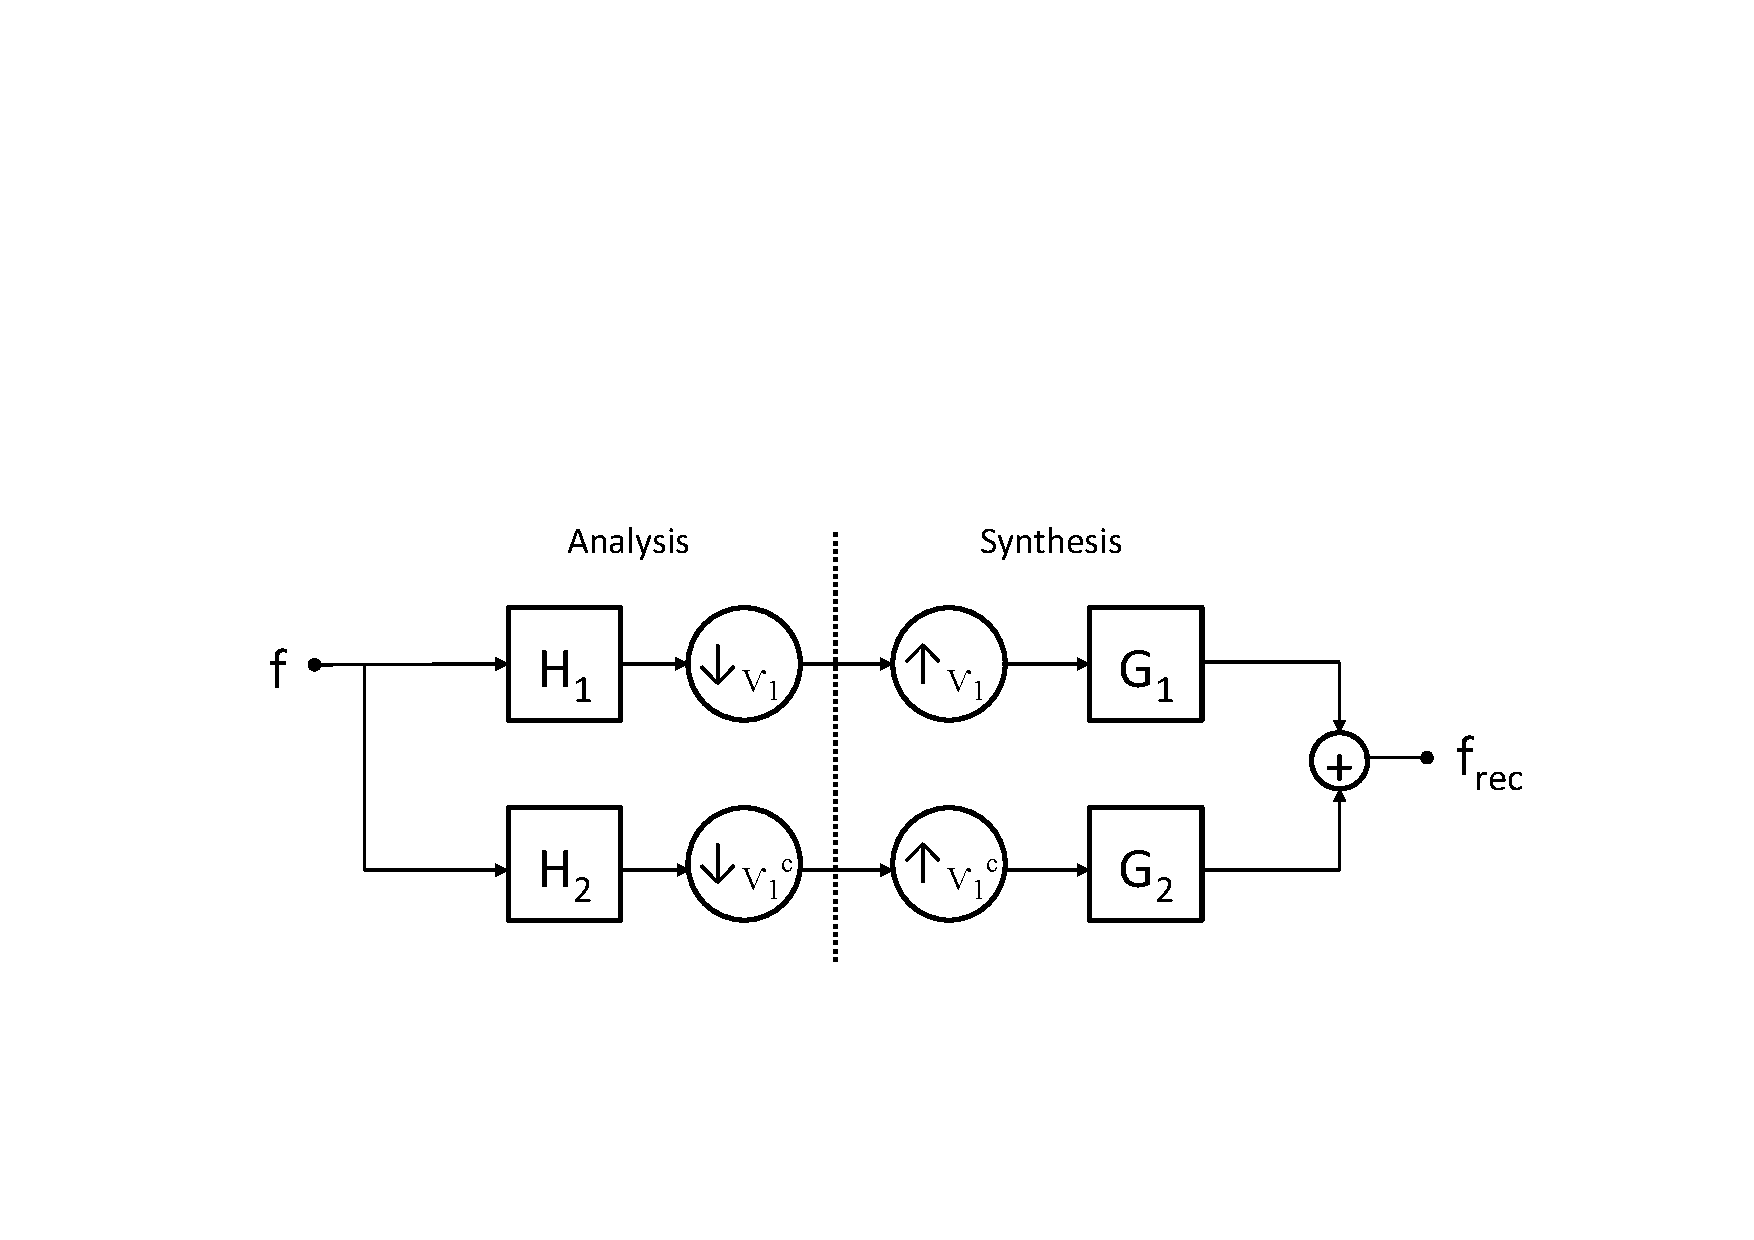
\includegraphics[width=3.3in]{fig_two_channel_classical}}
\caption{Extension of the classical two channel critically sampled filter bank to the graph setting. Here, $\mathbf{H}_1$ is a lowpass graph spectral filter, and $\mathbf{H}_2$ is a highpass graph spectral filter.}\label{Fig:two_channel}
\end{figure}


The extension of the classical two channel critically sampled filter bank to the graph setting was first proposed in \cite{narang_icip}. Fig.\ \ref{Fig:two_channel} shows the analysis and synthesis banks, where $H_i$ and $G_i$ are graph spectral filters \cite{shuman2013emerging}, and the lowpass and highpass bands are downsampled on complementary sets of vertices. For a general weighted, undirected graph, it is not straightforward %{\color{red} (impossible?)} 
how to design the downsampling and the four graph spectral filters to ensure perfect reconstruction. One approach is to separate the graph into a union of subgraphs, each of which has some regular structure. For example, \cite{narang2012perfect,narang_bior_filters} show that the normalized graph Laplacian eigenvectors of \emph{bipartite} graphs have a spectral folding property that make it possible to design analysis and synthesis filters to guarantee perfect reconstruction. They take advantage of this property by decomposing the graph into bipartite graphs and constructing a multichannel, separable filter bank, while \cite{sakiyama} adds vertices and edges to the original graph to form an approximating bipartite graph. References \cite{teke2016,teke2017ii} generalize this spectral folding property to $M$-block cyclic graphs, and leverage it to construct $M$-channel graph filter banks. Another class of regular structured graphs is \emph{shift invariant} graphs \cite[Chapter 5.1]{grady}. These graphs have a circulant graph Laplacian and their eigenvectors are the columns of the discrete Fourier transform matrix. Any graph can be written as the sum of circulant graphs, and \cite{ekambaram_icip,ekambaram2013globalsip,kotzagiannidis2016icassp} take advantage of this fact in designing critically sampled graph filter banks with perfect reconstruction. Another approach is to use architectures other than the critically sampled filter bank, such as lifting transforms \cite{jansen,narang_lifting_graphs} or pyramid transforms \cite{shuman_TSP_multiscale}.

Our approach in this paper is to replace the synthesis filters with interpolation operators on each subband of the graph spectrum. While this idea was initially suggested independently in \cite{chen2015discrete}, we investigate it in more detail here. Our construction leverages the recent flurry of work in sampling and reconstruction of graph signals \cite{chen2015discrete}-\nocite{pesenson_paley,narang2013interpolation,anis2014towards,gadde2015probabilistic,shomorony,PuyTGV15,chen2015signal,tsitsvero2016uncertainty}\cite{anis2016efficient}. The key property we use is that any signal whose graph Fourier transform has exactly $k$ non-zero coefficients can be perfectly recovered from samples of that signal on $k$ appropriately selected vertices (see, e.g., \cite[Theorem 1]{chen2015discrete} \cite[Proposition 1]{anis2016efficient}).

{\color{red} Add to intro here: scalable issues, outline, and contribution relative to conference paper.}


\section{$M$-Channel Critically Sampled Filter Bank}
We consider graph signals $f \in \R^N$ residing on a weighted, undirected graph $\G=\{\V,\E,\mathbf{W}\}$, where $\V$ is the set of $N$ vertices, $\E$ is the set of edges, and $\mathbf{W}$ is the weighted adjacency matrix. 
Throughout, we take $\L$ to be the combinatorial graph Laplacian $\mathbf{D}-\mathbf{W}$, where $\mathbf{D}$ is the diagonal matrix of vertex degrees. However, our theory and proposed transform also apply to the normalized graph Laplacian $\mathbf{I}-\mathbf{D}^{-\frac{1}{2}}\mathbf{W}\mathbf{D}^{-\frac{1}{2}}$, or any other Hermitian operator. We can diagonalize the graph Laplacian as $\L=\mathbf{U}{\boldsymbol \Lambda}\mathbf{U}^{*}$, where ${\boldsymbol \Lambda}$ is the diagonal matrix of eigenvalues $\lambda_0,\lambda_1,\ldots,\lambda_{N-1}$ of $\L$, and the columns $u_0,u_1,\ldots,u_{N-1}$ of $\mathbf{U}$ are the associated eigenvectors of $\L$. The graph Fourier transform of a signal is $\hat{f}=\mathbf{U}^{*}f$, and $\hat{g}(\L)f=\mathbf{U}\hat{g}({\boldsymbol \Lambda})\mathbf{U}^{*}f$ filters a graph signal by $\hat{g}(\cdot)$. We use the notation $\mathbf{U}_{{\cal R}}$ to denote the submatrix formed by taking the columns of $\mathbf{U}$ associated with the Laplacian eigenvalues indexed by ${\cal R} \subseteq \{0,1,\ldots,N-1\}$. Similarly, we use the notation $\mathbf{U}_{{\cal S},{\cal R}}$ to denote the submatrix  formed by taking the rows of $\mathbf{U}_{{\cal R}}$ associated with the vertices indexed by the set ${\cal S} \subseteq \{1,2,\ldots,N\}$.

We start by constructing an ideal filter bank of $M$ graph spectral filters, where each filter $\hat{h}_m(\lambda)$ is equal to 1 on a subset of the spectrum, and 0 elsewhere. We choose the filters so that for each $\l \in \{0,1,\ldots,N-1\}$, $\hat{h}_m(\lambda_\l)=1$ for exactly one $m$. Fig.\ \ref{Fig:fb} shows an example of such an ideal filter bank. Equivalently, we are forming a partition $\{{\cal R}_1,{\cal R}_2,\ldots,{\cal R}_M\}$ of $\{0,1,\ldots,N-1\}$ and setting 

\begin{figure}[t]
\centerline{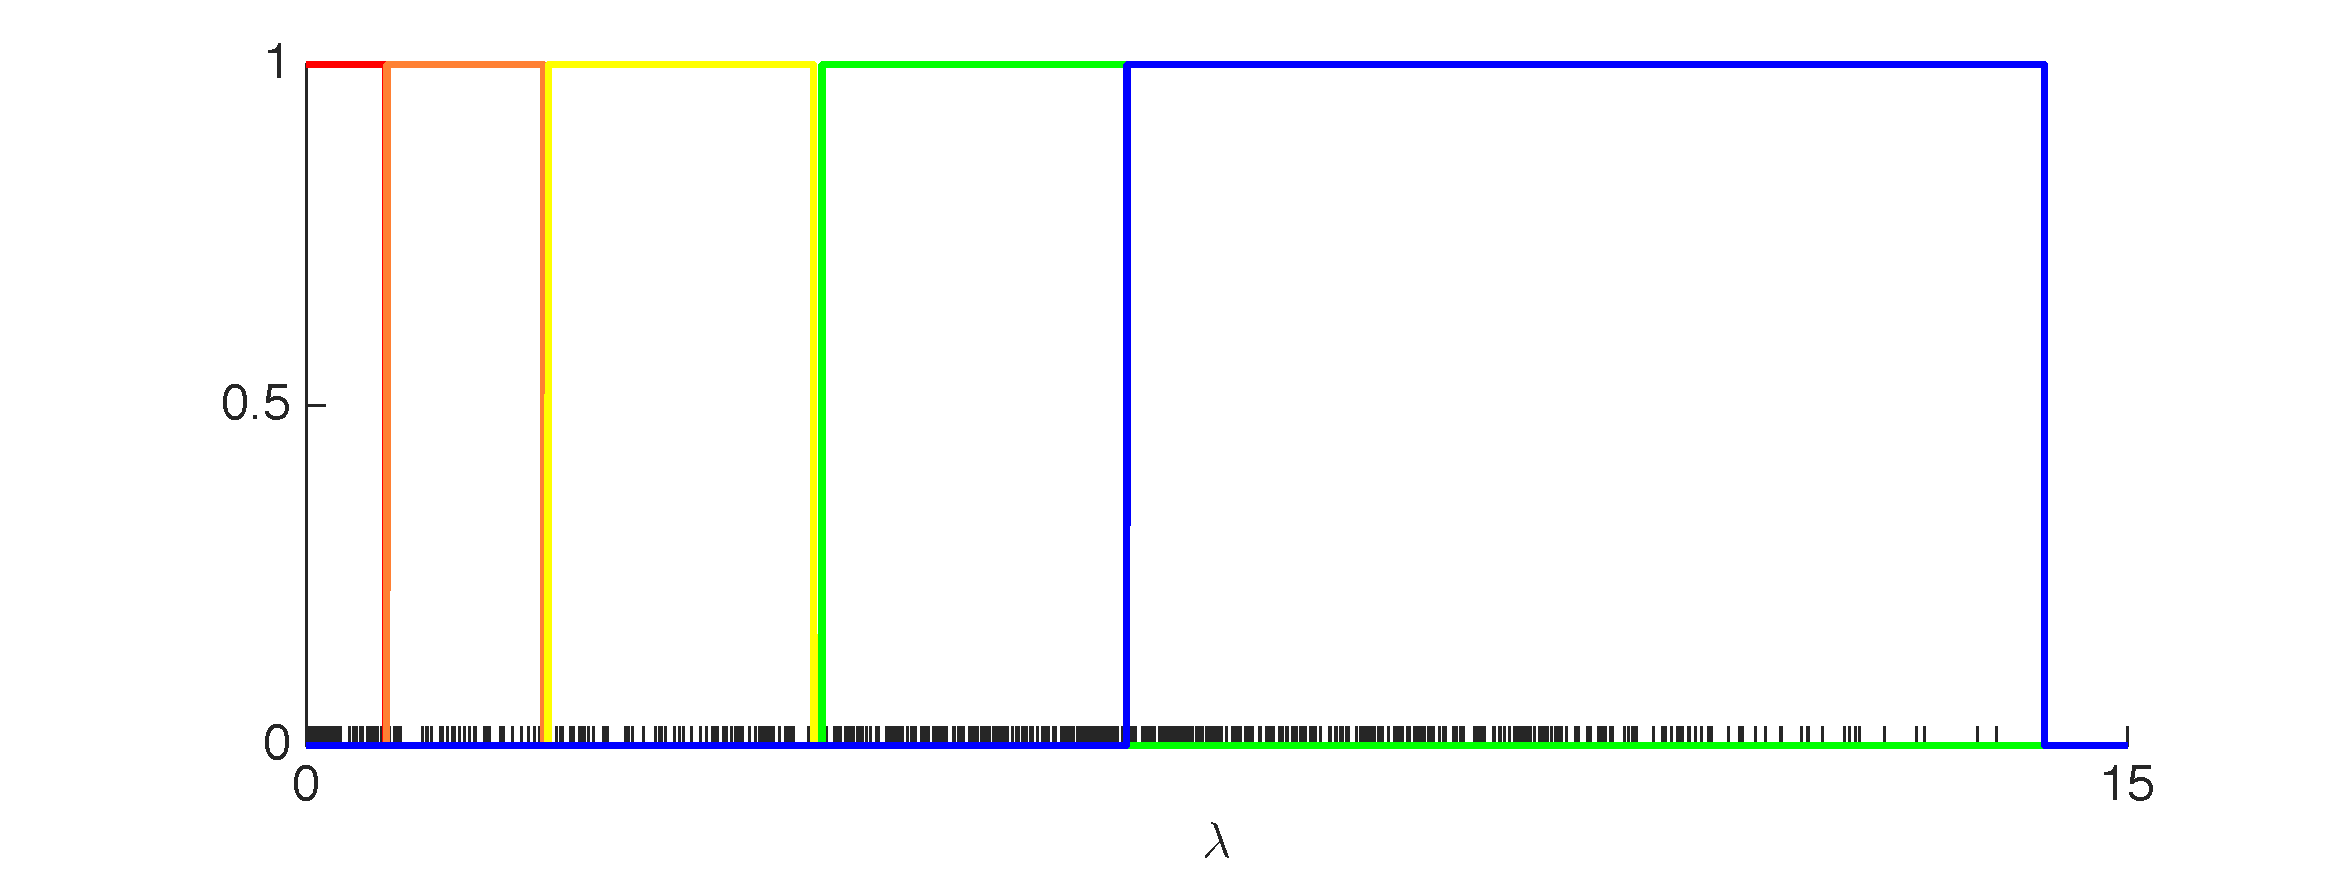
\includegraphics[width=3.1in]{fig_filter_bank}}
\caption{Example ideal filter bank. The red, orange, yellow, green, and blue filters span 31, 31, 63, 125, and 250 graph Laplacian eigenvalues, respectively, on a 500 node sensor network with %500 vertices and 
a maximum graph Laplacian eigenvalue of 14.3. The tick marks on the x-axis represent the locations of the graph Laplacian eigenvalues.}\label{Fig:fb}
\end{figure}

The next step, which we discuss in detail in the next section, is to partition the vertex set $\V$ into subsets $\V_1,\V_2,\ldots,\V_M$ such that $\V_m$ forms a uniqueness set for $\mbox{col}\left(\mathbf{U}_{{\cal R}_m}\right)$.
%the subband ${\cal R}_m$. 
\begin{definition}[Uniqueness set \cite{pesenson_paley}] 
%Let $${\cal R}=\{r_1,r_2,\ldots,r_K\} \subseteq \{0,1,\ldots,N-1\}$$ be a subset of the graph Laplacian eigenvalue indices. 
Let ${\cal P}$ be a subspace of $\R^n$. 
Then a subset $\V_s$ of the vertices $\V$ is a uniqueness set for 
%the subspace $\mbox{col}\left({\mathbf{U}}_{{\cal R}}\right)=\mbox{span}\{u_{r_1},u_{r_2}\ldots,u_{r_K}\} \subseteq \R^n$ 
${\cal P}$ if  and only if for all %$f,g \in \mbox{col}\left({\mathbf{U}}_{{\cal R}}\right)$, 
$f,g \in {\cal P}$,
$f_{\V_s}=g_{\V_s}$ implies $f=g$. That is, if two signals in ${\cal P}$ have the same values on the vertices in the uniqueness set $\V_s$, then they must be the same signal.
\end{definition}
The following equivalent characterization of a uniqueness set is often useful.
\begin{lemma}[\cite{anis2014towards}, \cite{shomorony}]\label{Le:eq_uniq}
The set $\mathcal{S}$ of $k$ vertices is a uniqueness set for $\mbox{col}({\mathbf{U}}_{\mathcal T})$ if and only if the matrix whose columns are $u_{{\mathcal T}_1},u_{{\mathcal T}_2},\ldots,u_{{\mathcal T}_k}, \delta_{{\mathcal{S}}^c_1}, \delta_{{\mathcal{S}}^c_2}, \ldots, \delta_{{\mathcal{S}}^c_{n-k}}$ is nonsingular,
where each $\delta_{{\mathcal{S}}^c_i}$ is a Kronecker delta centered on a vertex not included in $S$. 
\end{lemma}
The $m^{th}$ channel of the analysis %filter 
bank %then 
filters the graph signal by an ideal %low pass 
filter on subband ${\cal R}_m$, and downsamples the result onto the vertices in $\V_m$. For synthesis, we can interpolate from the samples on $\V_m$ to $\mbox{col}\left(\mathbf{U}_{{\cal R}_m}\right)$. If there is no error in the coefficients, then the reconstruction is perfect, because $\V_m$ is a uniqueness set for $\mbox{col}\left(\mathbf{U}_{{\cal R}_m}\right)$. Fig.\ \ref{Fig:arch} shows the architecture of the proposed $M$-channel critically sampled filter bank with interpolation on the synthesis side.

\begin{figure}[t]
\centerline{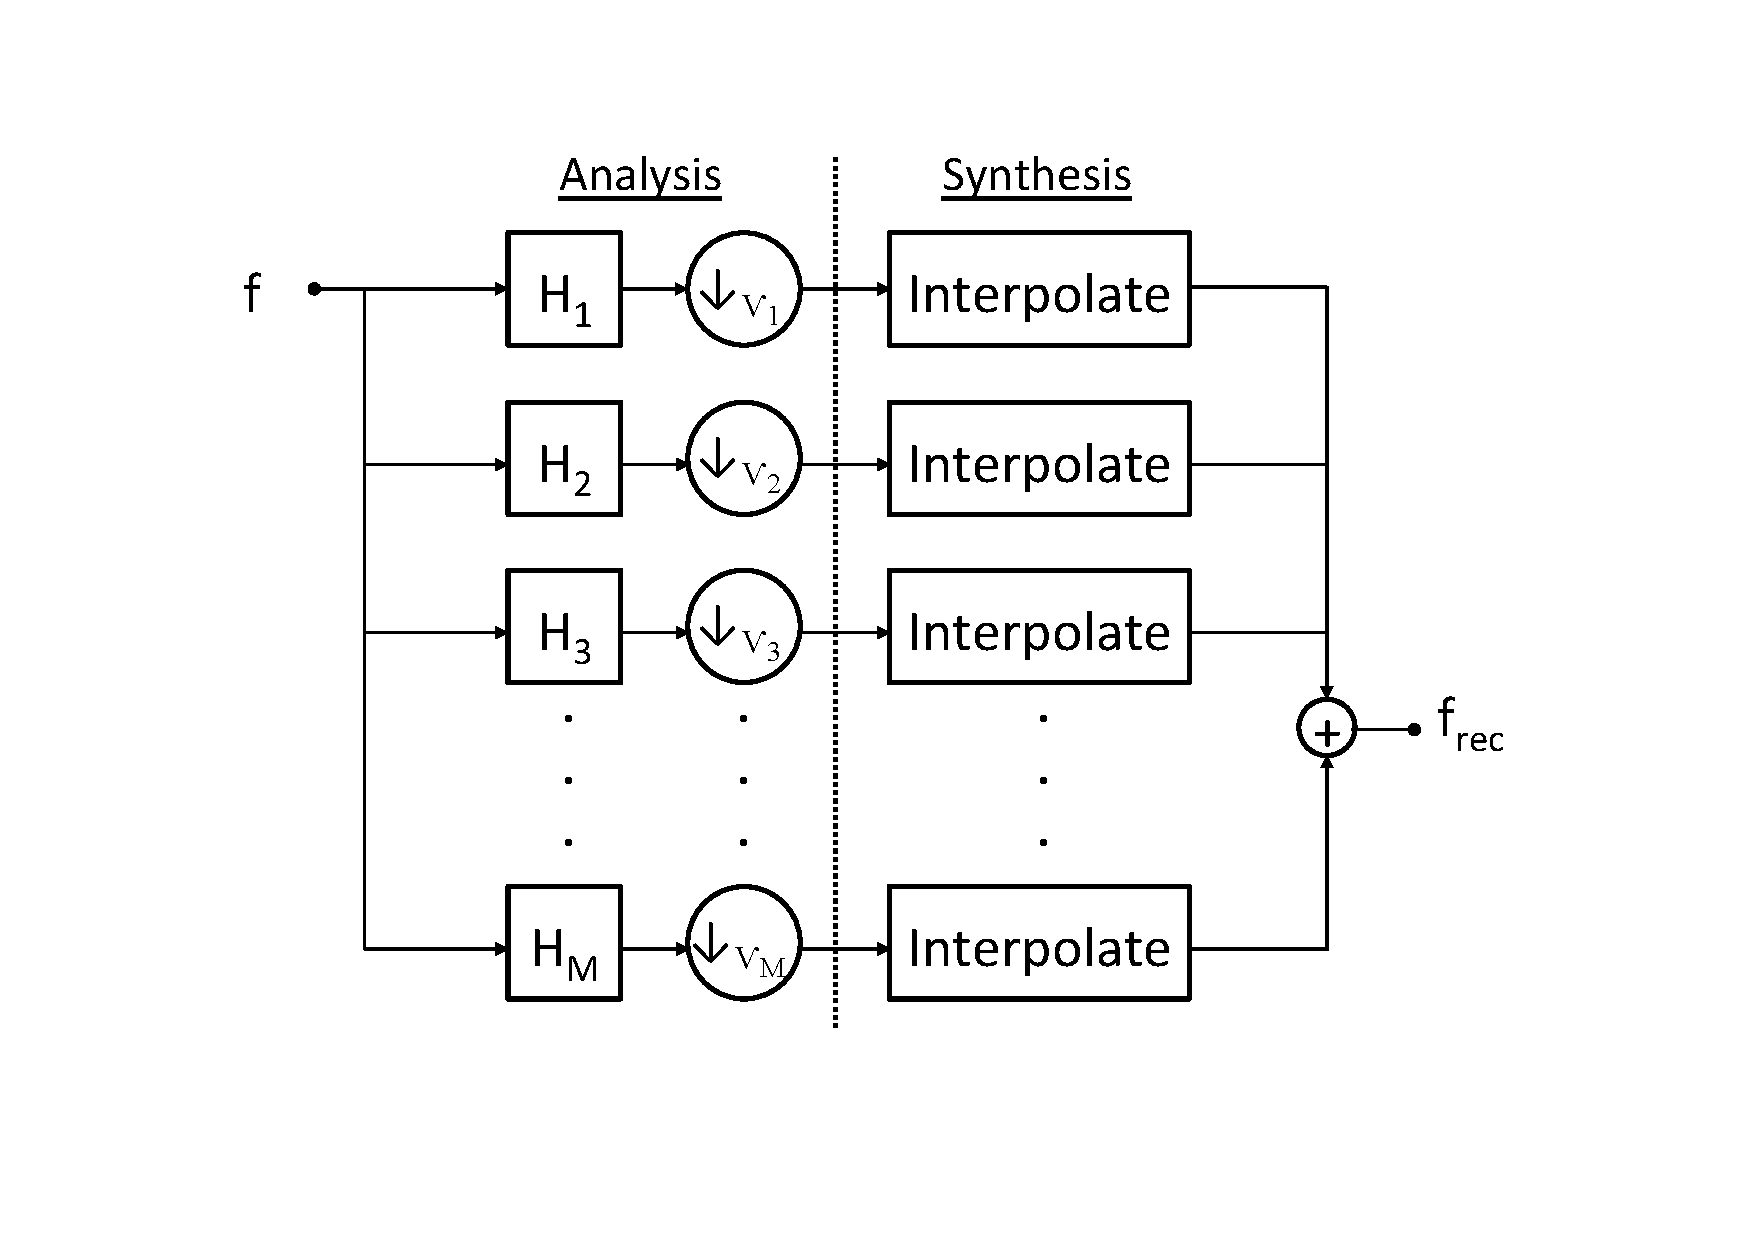
\includegraphics[width=2.8in]{fig_mcsfb_structure3}}
\caption{The $M$-channel critically sampled filter bank architecture. The sets $\V_1, \V_2, \ldots,\V_M$ form a partition of the set $\V$ of vertices, where each set $\V_m$ is a uniqueness set for graph signals supported on a different subband in the graph spectral domain.}\label{Fig:arch}
\end{figure}




\section{Partitioning the Graph into Uniqueness Sets for Different Frequency Bands}\label{Se:partition}

In this section, we show how to partition the set of vertices into uniqueness sets for different subbands of the graph Laplacian eigenvectors. We start with the easier case of $M=2$ and then examine the general case.

\subsection{$M=2$ channels}
%easier result that i
First we show that if a set of vertices is a uniqueness set for a set of signals contained in a band of spectral frequencies, then the complement set of vertices is a uniqueness set for the set of signals with no energy in that band of spectral frequencies.
\begin{proposition}\label{Le:highpass_uniqueness}
On a graph ${\mathcal G}$ with $N$ vertices, let 
${\mathcal T} \subseteq \{0,1,\ldots,N-1\}$ denote a subset of the graph Laplacian eigenvalue indices, and let ${\mathcal T}^c=\{0,1,\ldots,N-1\} \setminus {\mathcal T}$.
Then 
$\mathcal{S}^c$ is a uniqueness set for $\mbox{col}({\mathbf{U}}_{{\mathcal T}^c})$
 if and only if
$\mathcal{S}$ is a uniqueness set for 
$\mbox{col}({\mathbf{U}}_{{\mathcal T}})$.
\end{proposition}
This fact follows from either the CS decomposition \cite[Equation (32)]{paige})
%of C.C. Paige and M. Wei, "History and generality of the CS decomposition," Linear Algebra and Its Applications, 1992), 
or the nullity theorem \cite[Theorem 2.1]{strangInterplay}.  
%of G. Strang and T. Nguyen, "The interplay of ranks and submatrices," SIAM Review, 2004). 
We also provide a standalone proof below that only requires that the space spanned by the first $k$ columns of ${\mathbf{U}}$ is orthogonal to the space spanned by the last $N-k$ columns, not that ${\mathbf{U}}$ is an orthogonal matrix.

\begin{proof}[Proof of Proposition \ref{Le:highpass_uniqueness}]
We assume without loss of generality that ${\mathcal T}=\{0,1,2,\ldots,k-1\}$. 
Suppose first that the set $\mathcal{S}$ is a uniqueness set for $\mbox{col}({\mathbf{U}}_{\mathcal T})$, but $\mathcal{S}^c$ is not a uniqueness set for $\mbox{col}({\mathbf{U}}_{{\mathcal T}^c})$. Then by Lemma \ref{Le:eq_uniq}, the matrix $$\mathbf{A}=
 \left[ \begin{array}{cccccccc}
u_{0} & u_{1} & \cdots & u_{k-1} & \delta_{{\mathcal{S}}^c_1} & \delta_{{\mathcal{S}}^c_2} \cdots & \delta_{{\mathcal{S}}^c_{N-k}} \end{array} \right]$$
has full rank, and the matrix $$\mathbf{B}=
 \left[ \begin{array}{cccccccc}
u_{k} & u_{k+1} & \cdots & u_{N-1} & \delta_{\mathcal{S}_{1}} & \delta_{\mathcal{S}_{2}} \cdots & \delta_{\mathcal{S}_k} \end{array} \right]$$
is singular, implying
\begin{align}\label{Eq:span}
\mbox{span}(u_{k}, u_{k+1},\ldots, u_{N-1}, \delta_{\mathcal{S}_{1}}, \delta_{\mathcal{S}_{2}}, \ldots, \delta_{\mathcal{S}_k}) \neq \mathbb{R}^N.
\end{align}
Since 
$$\mbox{dim}(\mbox{span}(u_{k}, u_{k+1},\ldots, u_{N-1}))=N-k$$ and $$\mbox{dim}(\mbox{span}(\delta_{S_{1}}, \delta_{S_{2}}, \ldots, \delta_{\mathcal{S}_k}))=k,$$ equation 
\eqref{Eq:span} implies that
there must exist a vector $x \neq 0$ such that 
\begin{align*}
&x \in  \mbox{span}(u_{k}, u_{k+1},\ldots, u_{N-1})  \hbox{ and } \\
& x \in \mbox{span}(\delta_{\mathcal{S}_{1}}, \delta_{\mathcal{S}_{2}}, \ldots, \delta_{\mathcal{S}_{k}}).\end{align*}
Yet, $x \in \mbox{col}({\mathbf{U}}_{{\mathcal T}^c})$ implies $x$ is orthogonal to  $u_0, u_1, \ldots, u_{k-1}$, and, similarly, 
$x \in \mbox{span}(\delta_{\mathcal{S}_{1}}, \delta_{\mathcal{S}_{2}}, \ldots, \delta_{\mathcal{S}_{k}})$ implies $x$ is orthogonal to $\delta_{\mathcal{S}^c_{1}}, \delta_{\mathcal{S}^c_{2}}, \ldots, \delta_{\mathcal{S}^c_{N-k}}.$
In matrix notation, we have $\mathbf{A}^{\top}x=0$, so $\mathbf{A}^{\top}$ has a non-trivial null space, and thus the square matrix $\mathbf{A}$ is not full rank and $\mathcal{S}$ is not a uniqueness set for $\mbox{col}({\mathbf{U}}_{\mathcal T})$, a contradiction. We conclude that if $\mathbf{A}$ is full rank, then $\mathbf{B}$ must be full rank and $\mathcal{S}^c$ is a uniqueness set for $\mbox{col}({\mathbf{U}}_{{\mathcal T}^c})$, completing the proof of sufficiency. Necessity follows from the same argument, with the roles of $\mathbf{A}$ and $\mathbf{B}$ interchanged.
\end{proof}

The Steinitz exchange lemma \cite{steinitz} guarantees that we can find the uniqueness set $\mathcal{S}$ (and thus $\mathcal{S}^c$), and the graph signal processing literature contains methods such as Algorithm 1 of \cite{shomorony} to do so.

\subsection{$M>2$ channels}
The issue with using the methods of Proposition \ref{Le:highpass_uniqueness} for the case of $M>2$ is that while the submatrix ${\mathbf{U}}_{{\mathcal S^c},{\mathcal T^c}}$ is nonsingular, it is not necessarily orthogonal, and so we cannot proceed with an inductive argument. The following proposition and corollary circumvent this issue by only using the nonsingularity of the original matrix. The proof of the following proposition is due to Federico Poloni \cite{poloni}, %of the University of Pisa via mathoverflow.net
and we later discovered the same method in \cite{greeneMultiple}, \cite[Theorem 3.3]{greene_magnanti}.
\begin{proposition}\label{Pr:mat_part}
Let $\mathbf{A}$ be an $N \times N$ nonsingular matrix, and $\beta=\{\beta_1,\beta_2,\ldots,\beta_M\}$ be a partition of $\{1,2,\ldots,N\}$. Then there exists another partition $\alpha=\{\alpha_1,\alpha_2,\ldots,\alpha_M\}$ of $\{1,2,\ldots,N\}$ with $|\alpha_i|=|\beta_i|$ for all $i$ such that the $M$ square submatrices $\mathbf{A}_{\alpha_i,\beta_i}$ are all nonsingular.
\end{proposition}
\begin{proof}%[Proof of Proposition \ref{Pr:part_uniq}]
First consider the case $M=2$, and let $k=|\beta_1|$. Then by the generalized Laplace expansion \cite{gle}, 
\begin{align}\label{Eq:det2}
\mbox{det}(\mathbf{A})~=~\sum_{\mathclap{\{\alpha_1 \subset \{1,2,\ldots,N\}: |\alpha_1|=k \}}}~~\sigma_{\alpha_1,\beta_1} \mbox{det}(\mathbf{A}_{\alpha_1,\beta_1})\mbox{det}(\mathbf{A}_{\alpha_1^c,\beta_2}),
\end{align}
where the sign $\sigma_{\alpha_1,\beta_1}$ of the permutation determined by $\alpha_1$ and $\beta_1$ is equal to 1 or -1. Since $\mbox{det}(\mathbf{A})\neq 0$, one of the terms in the summation of \eqref{Eq:det2} must be nonzero, ensuring a choice of $\alpha_1$ such that the submatrices $\mathbf{A}_{\alpha_1,\beta_1}$ and $\mathbf{A}_{\alpha_1^c,\beta_2}$ are nonsingular. We can choose $\{\alpha_1,\alpha_1^c\}$ as the desired partition. For $M>2$, by induction, we have
\begin{align}\label{Eq:detM}
\mbox{det}(\mathbf{A})~=~\sum_{\mathclap{\{\hbox{Partitions } \alpha \hbox{ of }\{1,2,\ldots,N\}: |\alpha_i|=|\beta_i|~\forall i \}}}~~\sigma_{\alpha}~{\textstyle \prod_{i=1}^M}~\mbox{det}(\mathbf{A}_{\alpha_i,\beta_i}),
\end{align}
where again $\sigma_\alpha$ is always 1 or -1 and one of the terms in the summation in \eqref{Eq:detM} must be nonzero, yielding the desired partition. 
\end{proof}
\begin{corollary}\label{Co:part_uniq}
For any %arbitrary 
partition $\{{\cal R}_1,{\cal R}_2,\ldots {\cal R}_M \}$ of the graph Laplacian eigenvalue indices $\{0,1,\ldots,N-1\}$ into $M$ subsets, there exists a partition $\{\V_1,\V_2,\ldots,\V_M\}$ of the graph vertices into $M$ subsets 
such that for every $m \in \{1,2,\ldots,M\}$, $|\V_m|=|{\cal R}_m|$ and 
%of corresponding sizes such that each subset 
$\V_m$ is a uniqueness set for $\mbox{col}\left(\mathbf{U}_{{\cal R}_m}\right)$.%of the vertices is the uniqueness set for each of the bandwidth sets.
\end{corollary}
\begin{proof}
By Proposition \ref{Pr:mat_part}, we can find a partition such that $\mathbf{U}_{\V_m,{\cal R}_m}$ is nonsingular for all $m$. Let $\mathbf{E}_m$ be the matrix formed by joining the $k_m$ columns of  $\mathbf{U}$ indexed by ${\cal R}_m$ with $N-k_m$ Kronecker deltas centered on all vertices not included in $\V_m$. By Lemma \ref{Le:eq_uniq}, it suffices to show that the matrices $\mathbf{E}_m$ are all nonsingular. Yet, for all $m$, we have
$$|\mbox{det}(\mathbf{E}_m)|=|\mbox{det}(\mathbf{U}_{\V_m,{\cal R}_m})| \neq 0.$$
\end{proof}

Corollary \ref{Co:part_uniq} ensures the existence of the desired partition, and the proof of Proposition \ref{Pr:mat_part} suggests that we can find it inductively. However, given a partition of the columns of ${\mathbf{A}}$ into two sets $\mathcal{T}$ and $\mathcal{T}^c$, Proposition \ref{Pr:mat_part} does not provide a constructive method to partition the rows of ${\mathbf{A}}$ into two sets $\mathcal{S}$ and $\mathcal{S}^c$ such that the submatrices ${\mathbf{A}}_{{\mathcal{S}},{\mathcal{T}}}$ and ${\mathbf{A}}_{{\mathcal{S}^c},{\mathcal{T}}^c}$ are nonsingular. This problem is studied in the more general framework of matroid theory in \cite{greene_magnanti}, which gives an algorithm to find the desired row partition into two sets. We summarize this method in Algorithm \ref{Al:uniqueness}, which takes in a partition $\{{\cal R}_1,{\cal R}_2,\ldots {\cal R}_M \}$ of the spectral indices and constructs the partition $\{\V_1,\V_2,\ldots,\V_M\}$ of the vertices. In Fig. \ref{Fig:part_examples}, we show two examples of the resulting partitions.

\begin{algorithm} 
\caption{Partition the vertices into uniqueness sets for each frequency band}
\begin{algorithmic}
\State \textbf{Input} $\mathbf{U}$,~a partition $\{{{\cal R}_1,{\cal R}_2,\ldots,{\cal R}_M}\}$ %of the spectrum %, a partition of $\{0,1,\ldots,N-1\}$
\State $\mathcal{S} \gets \emptyset$
%\State $\mathcal{R} \gets \emptyset$
\For {$m=1,2,\ldots,M$}%{each frequency set ${\cal R}_m$}
\State Find sets $\gamma_1, \gamma_2 \subset {\mathcal{S}}^c$ s.t. $\mathbf{U}_{\gamma_1,{\cal R}_m}$ and $\mathbf{U}_{\gamma_2,{\cal R}_{m+1:M}}$ are nonsingular
\While {$\gamma_1 \cap \gamma_2 \neq \emptyset$}
\State Find a chain of pivots from an element $y \in {\mathcal S}^c \setminus (\gamma_1 \cup \gamma_2)$
to an element $z \in \gamma_1 \cap \gamma_2$ (c.f. \cite{greene_magnanti} for details)
\State Update $\gamma_1$ and $\gamma_2$ by carrying out a series of exchanges resulting with $y$ and $z$ each appearing in exactly one of $\gamma_1$ or $\gamma_2$
\EndWhile
\State $\V_m \gets \gamma_1$%\V_m \cup v$
\State $\mathcal{S} \gets \mathcal{S} \cup \gamma_1$ % \V_m$
\EndFor
\State \textbf{Output} the partition $\{\V_1,\V_2,\ldots,\V_M$\}
\end{algorithmic}
\label{Al:uniqueness}
\end{algorithm}

\begin{remark}
While Algorithm \ref{Al:uniqueness} always finds a partition into uniqueness sets, such a partition is usually not unique, and the initial choices of $\gamma_i$ in each loop play a significant role in the final 
partition. In the numerical experiments in the next section, we use the greedy algorithm in \cite[Algorithm 1]{shomorony} to find an initial choice for $\gamma_1$, and use row reduction after permuting the complement of $\gamma_1$ to the top to find an initial choice for $\gamma_2$. We discuss this issue further in Section \ref{Se:noisy_ext}.
\end{remark}

\begin{figure}[tb]
\begin{minipage}[m]{0.43\linewidth}
\centerline{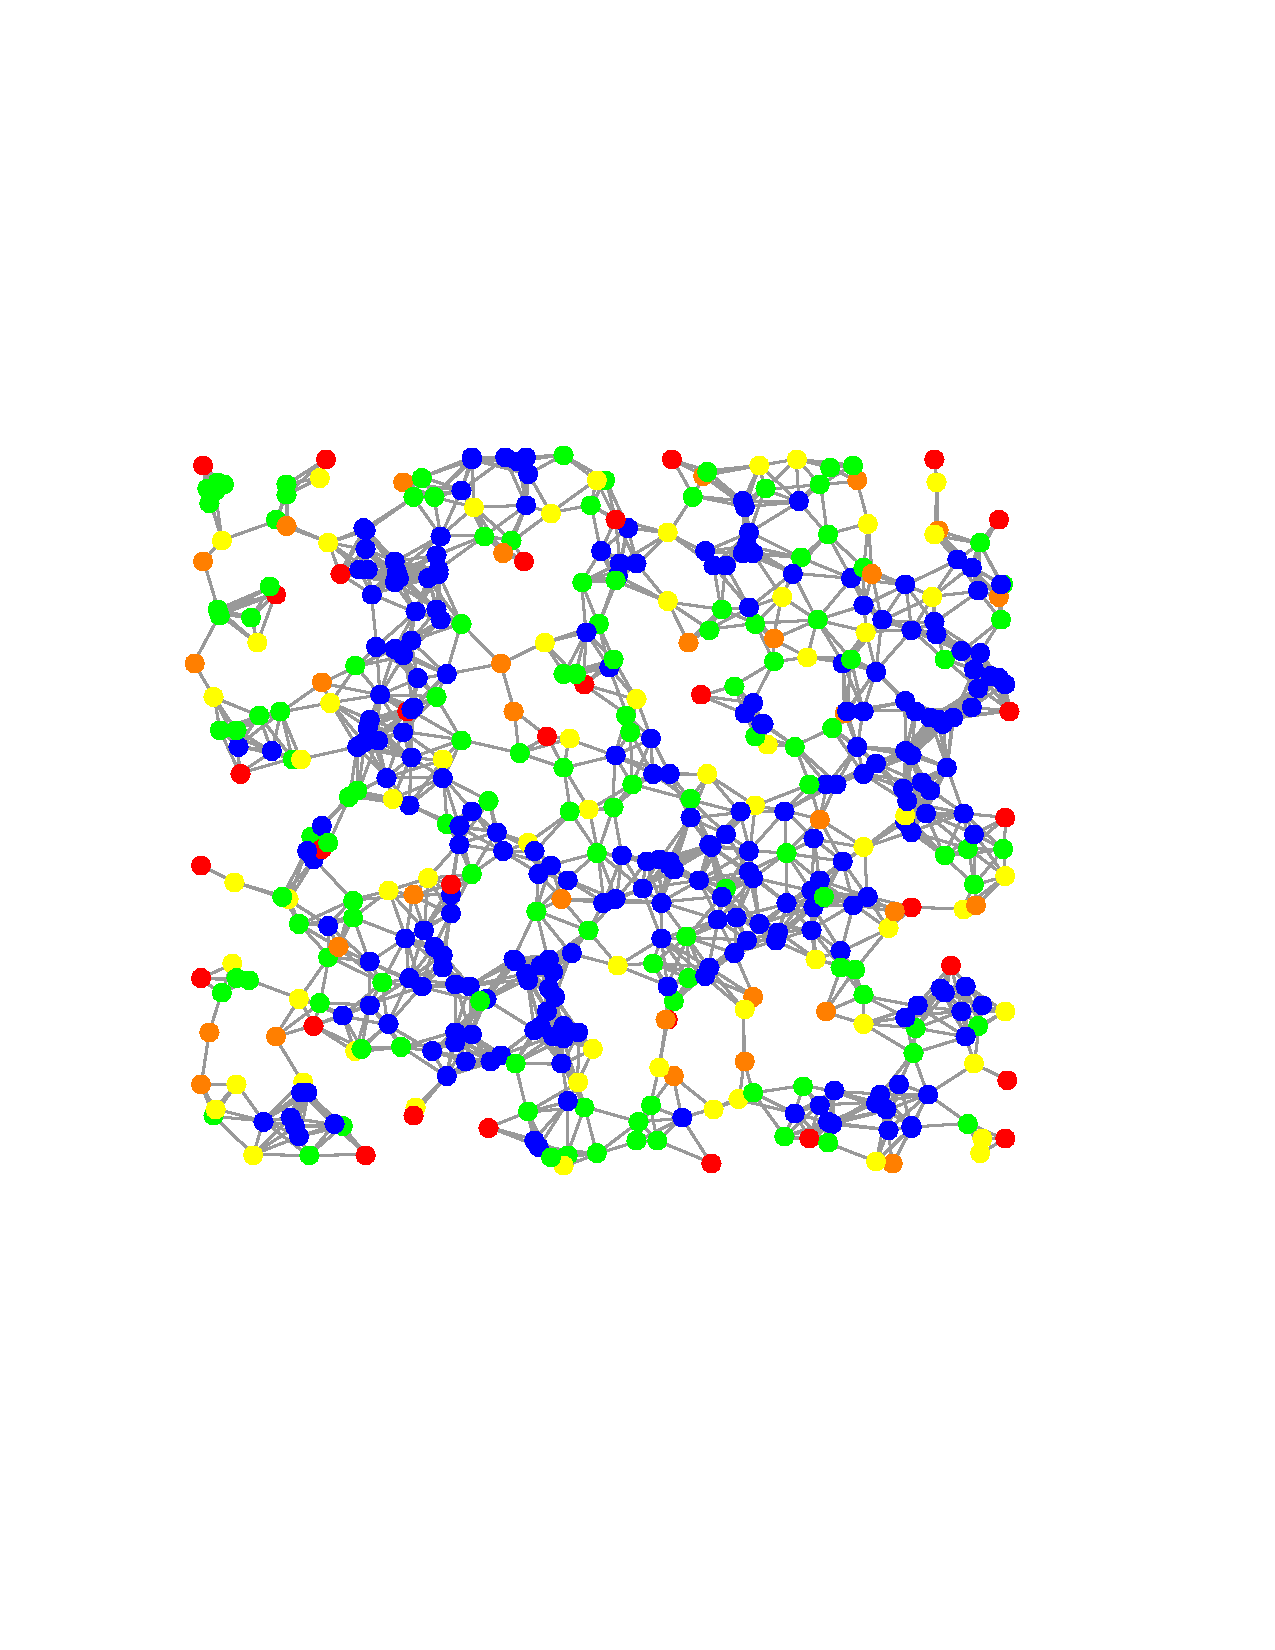
\includegraphics[width=.98\linewidth]{fig_uniq_part_sensor3}}
\end{minipage}
\hspace{.003\linewidth}
\begin{minipage}[m]{0.05\linewidth}
\centerline{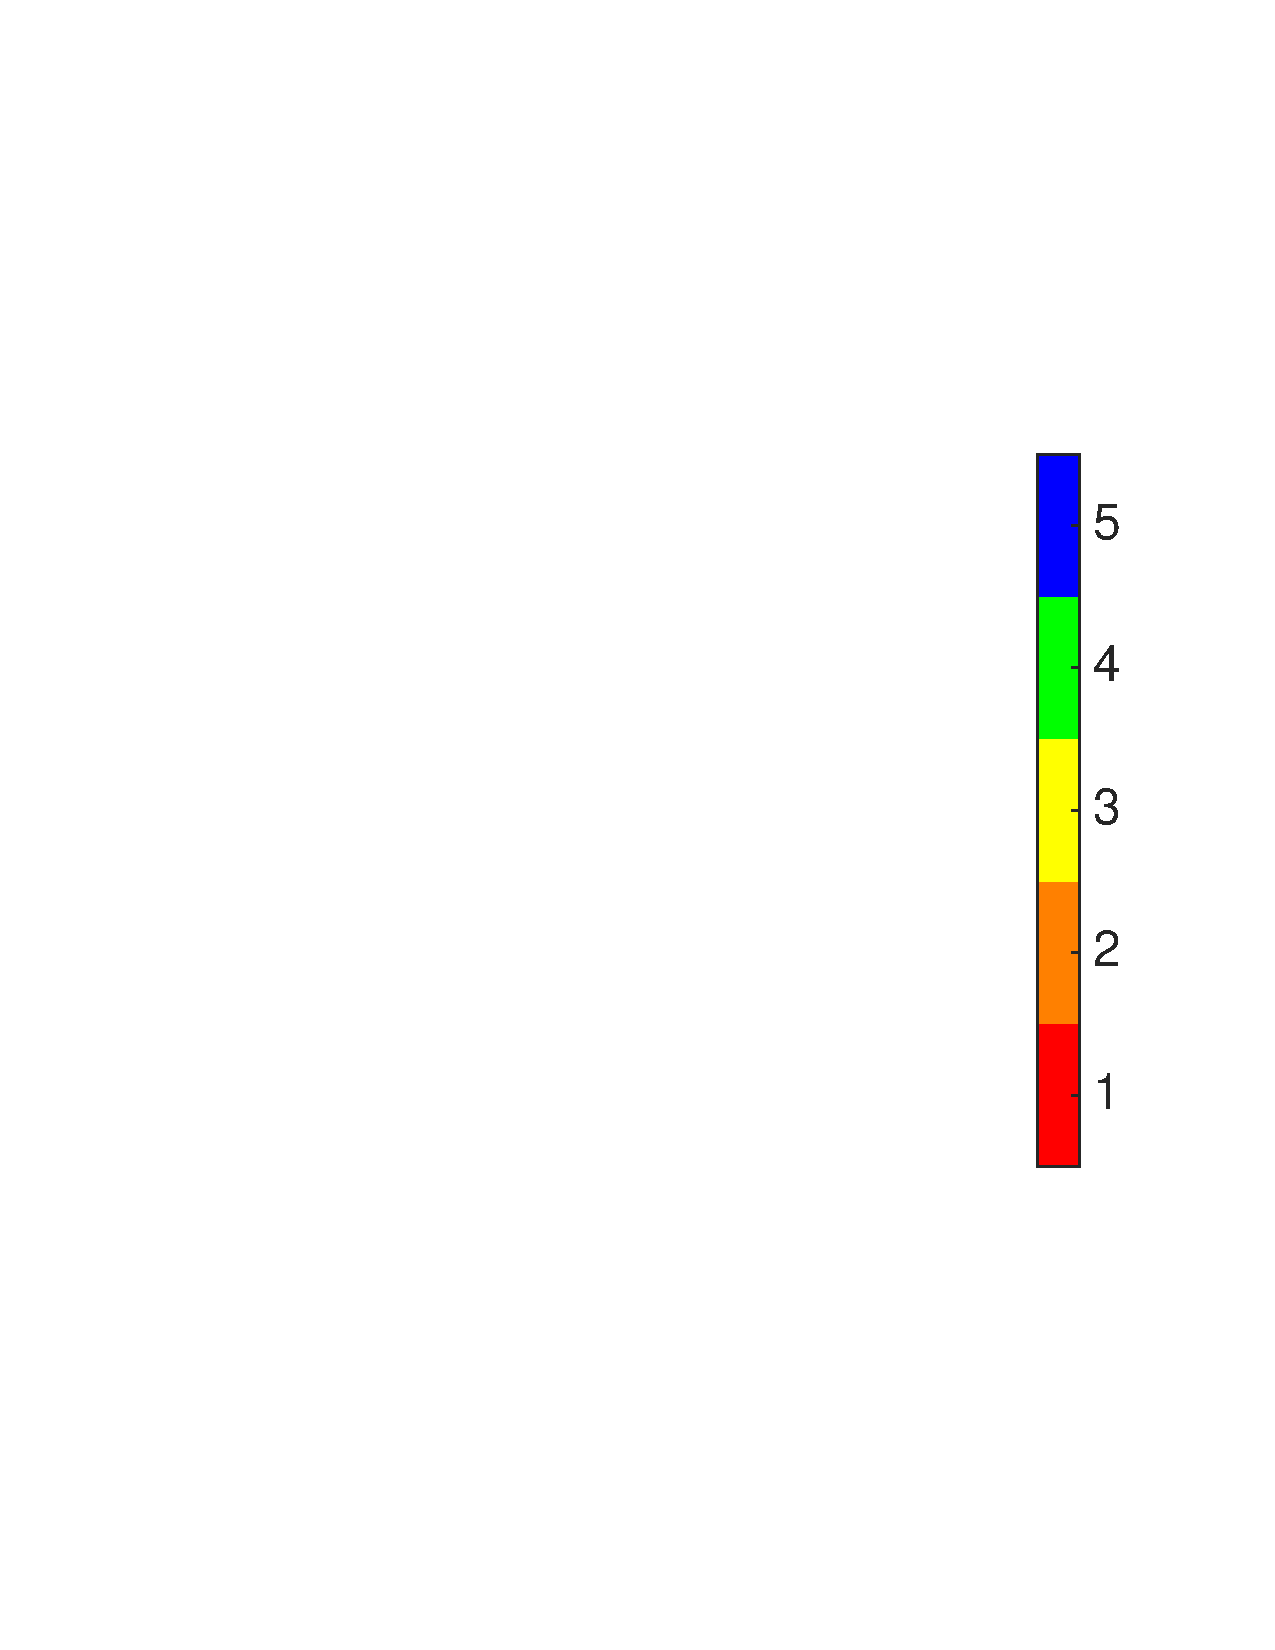
\includegraphics[width=.9\linewidth]{fig_uniq_part_col2}}
\end{minipage}
\hspace{.003\linewidth}
\begin{minipage}[m]{0.46\linewidth}
\centerline{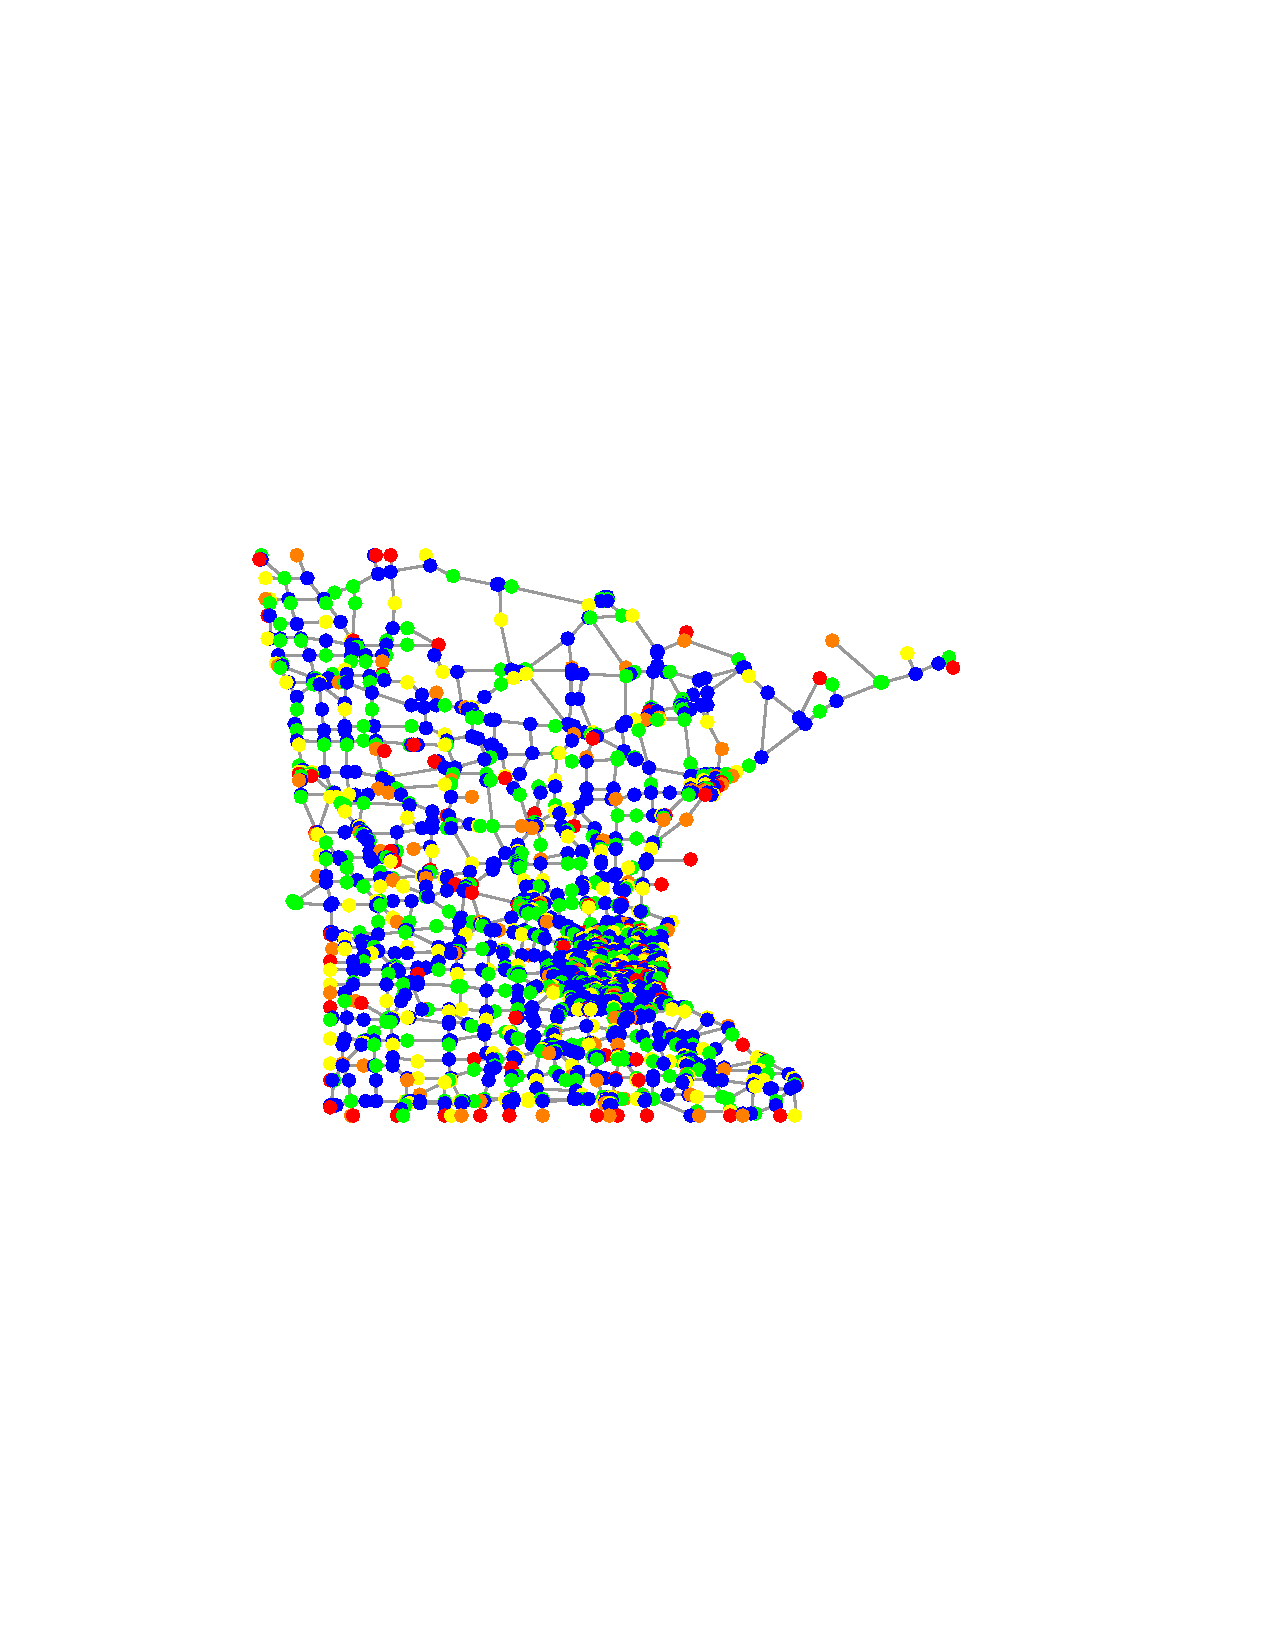
\includegraphics[width=\linewidth]{fig_uniq_part_minn4}}
\end{minipage}
\caption{Partitions of a 500 node random sensor network and the Minnesota road network \cite{gleich} into uniqueness sets for five different spectral bands, with the indices increasing from lowpass bands (1) to highpass bands (5).} \label{Fig:part_examples}
\end{figure} 

{\color{red}
\section{Signals that are Sparsely Represented by the MCSFB Transform}
\begin{itemize}
\item Add theorem about orthogonality across bands
\item Mention signals that are sparse
\item Characterization of joint localization?
\end{itemize}
}

\section{Illustrative Examples I: Exact Calculations}
We can represent the proposed filter bank as an $N \times N$ dictionary matrix $\boldsymbol{\Phi}$ that maps graph signals to their filter bank analysis coefficients. 

\begin{figure*}[bth] 
\begin{minipage}[m]{0.16\linewidth}
~
\end{minipage}
\begin{minipage}[m]{0.16\linewidth}
\centerline{\small{Scaling Functions}}
\end{minipage}
\hspace{.01\linewidth}
\begin{minipage}[m]{0.16\linewidth}
\centerline{\small{Wavelet Scale 1~~~~}}
\end{minipage}
\begin{minipage}[m]{0.16\linewidth}
\centerline{\small{Wavelet Scale 2~~~~}}\end{minipage}
\begin{minipage}[m]{0.16\linewidth}
\centerline{\small{Wavelet Scale 3~~~~}}\end{minipage}
\begin{minipage}[m]{0.16\linewidth}
\centerline{\small{Wavelet Scale 4~~~~~}}\end{minipage} \\
\begin{minipage}[m]{0.16\linewidth}
\centerline{\small{Example Atom}}
\end{minipage}
\begin{minipage}[m]{0.16\linewidth}
\centerline{~~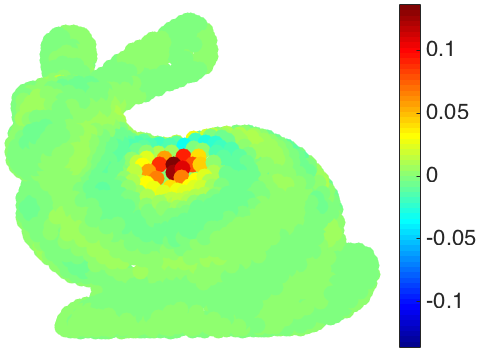
\includegraphics[width=.85\linewidth]{fig_bunny_atom_scalinga}}
\end{minipage}
\begin{minipage}[m]{0.16\linewidth}
\centerline{~~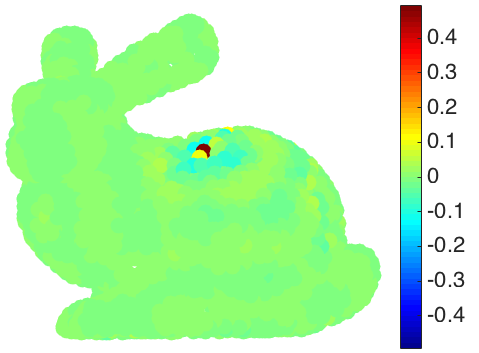
\includegraphics[width=.85\linewidth]{fig_bunny_atom_wav1a}}
\end{minipage}
\begin{minipage}[m]{0.16\linewidth}
\centerline{~~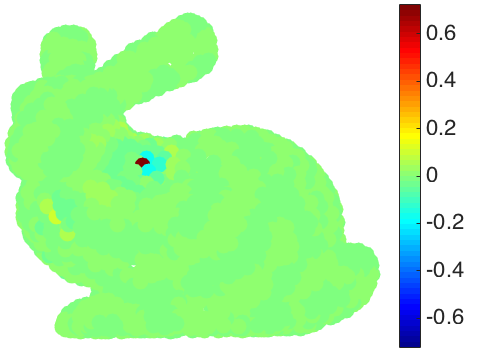
\includegraphics[width=.85\linewidth]{fig_bunny_atom_wav2a}}
\end{minipage}
\begin{minipage}[m]{0.16\linewidth}
\centerline{~~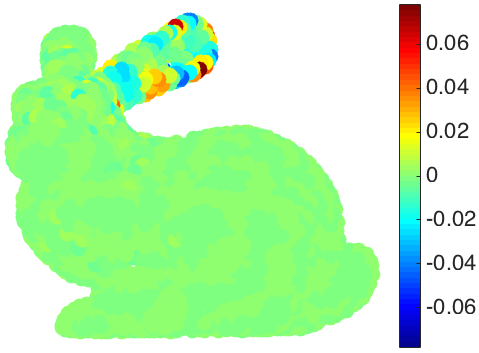
\includegraphics[width=.85\linewidth]{fig_bunny_atom_wav3a}}
\end{minipage}
\begin{minipage}[m]{0.16\linewidth}
\centerline{~~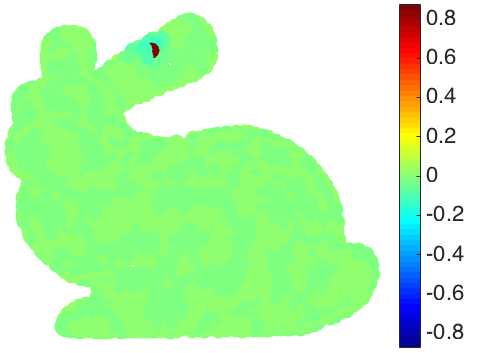
\includegraphics[width=.85\linewidth]{fig_bunny_atom_wav4a}}
\end{minipage}\\
\begin{minipage}[m]{0.16\linewidth}
\centerline{\small{Spectral Content}}
\centerline{\small{of All Atoms}}
\end{minipage}
\begin{minipage}[m]{0.16\linewidth}
\centerline{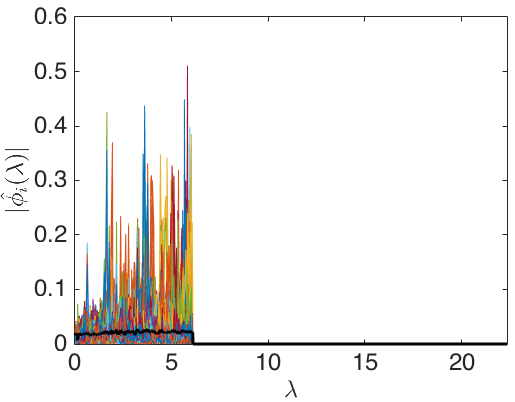
\includegraphics[width=.8\linewidth]{fig_bunny_freq_scaling3}}
\end{minipage}
\begin{minipage}[m]{0.16\linewidth}
\centerline{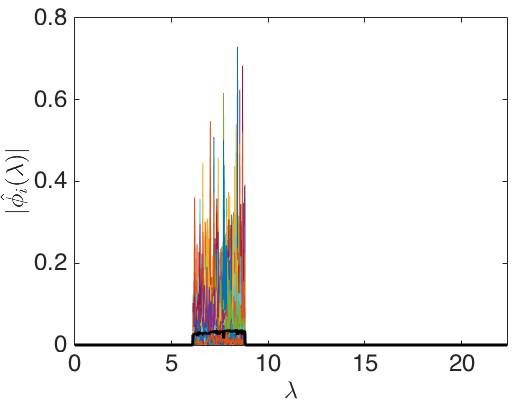
\includegraphics[width=.8\linewidth]{fig_bunny_freq_wav1a}}
\end{minipage}
\begin{minipage}[m]{0.16\linewidth}
\centerline{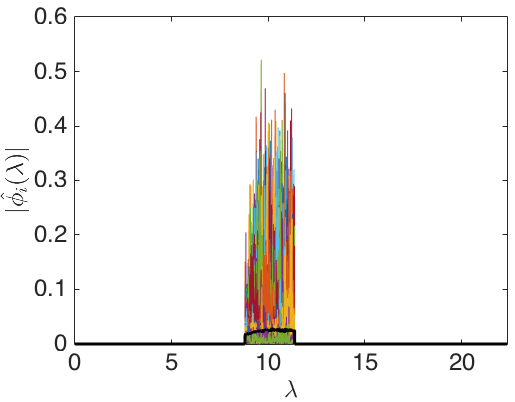
\includegraphics[width=.8\linewidth]{fig_bunny_freq_wav2a}}
\end{minipage}
\begin{minipage}[m]{0.16\linewidth}
\centerline{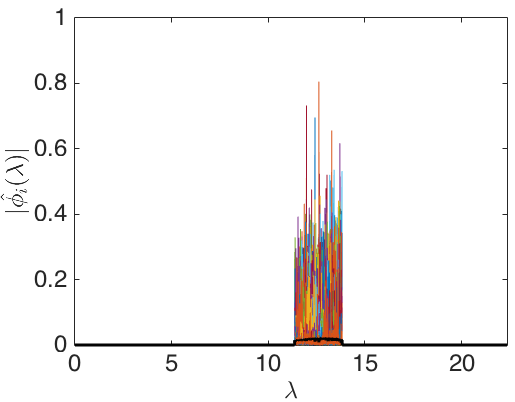
\includegraphics[width=.8\linewidth]{fig_bunny_freq_wav3a}}
\end{minipage}
\begin{minipage}[m]{0.16\linewidth}
\centerline{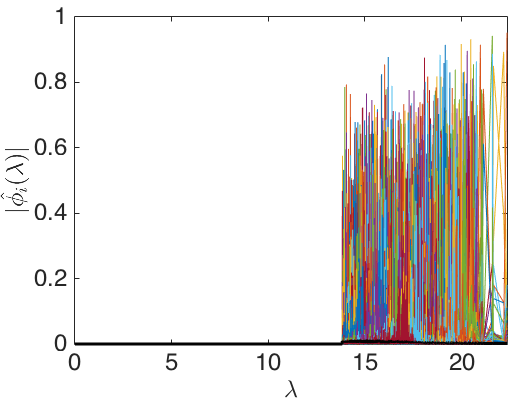
\includegraphics[width=.8\linewidth]{fig_bunny_freq_wav4a}}
\end{minipage}\\
\begin{minipage}[m]{0.16\linewidth}
\centerline{\small{Analysis}}
\centerline{\small{Coefficients}}
\end{minipage}
\begin{minipage}[m]{0.16\linewidth}
\centerline{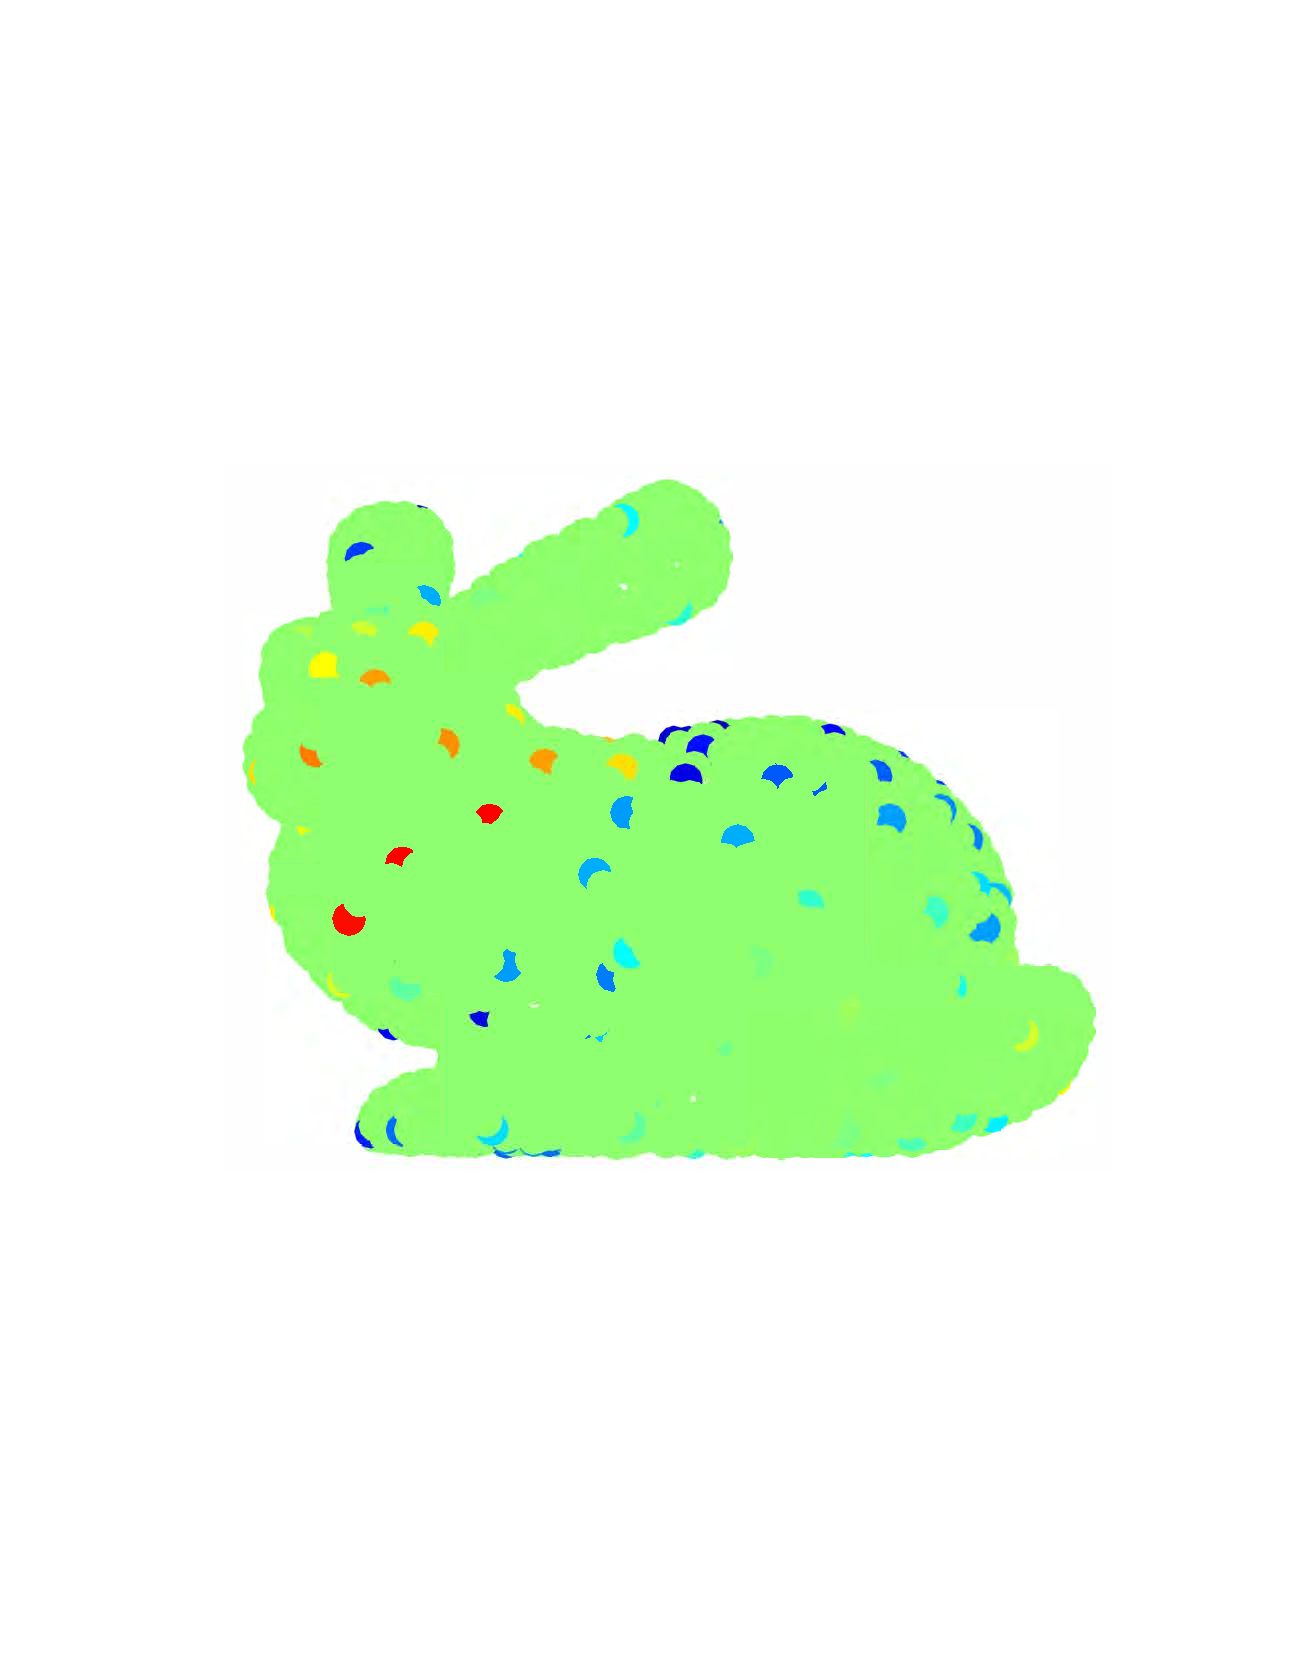
\includegraphics[width=.8\linewidth]{fig_bunny_coef_scaling}}
\end{minipage}
\begin{minipage}[m]{0.16\linewidth}
\centerline{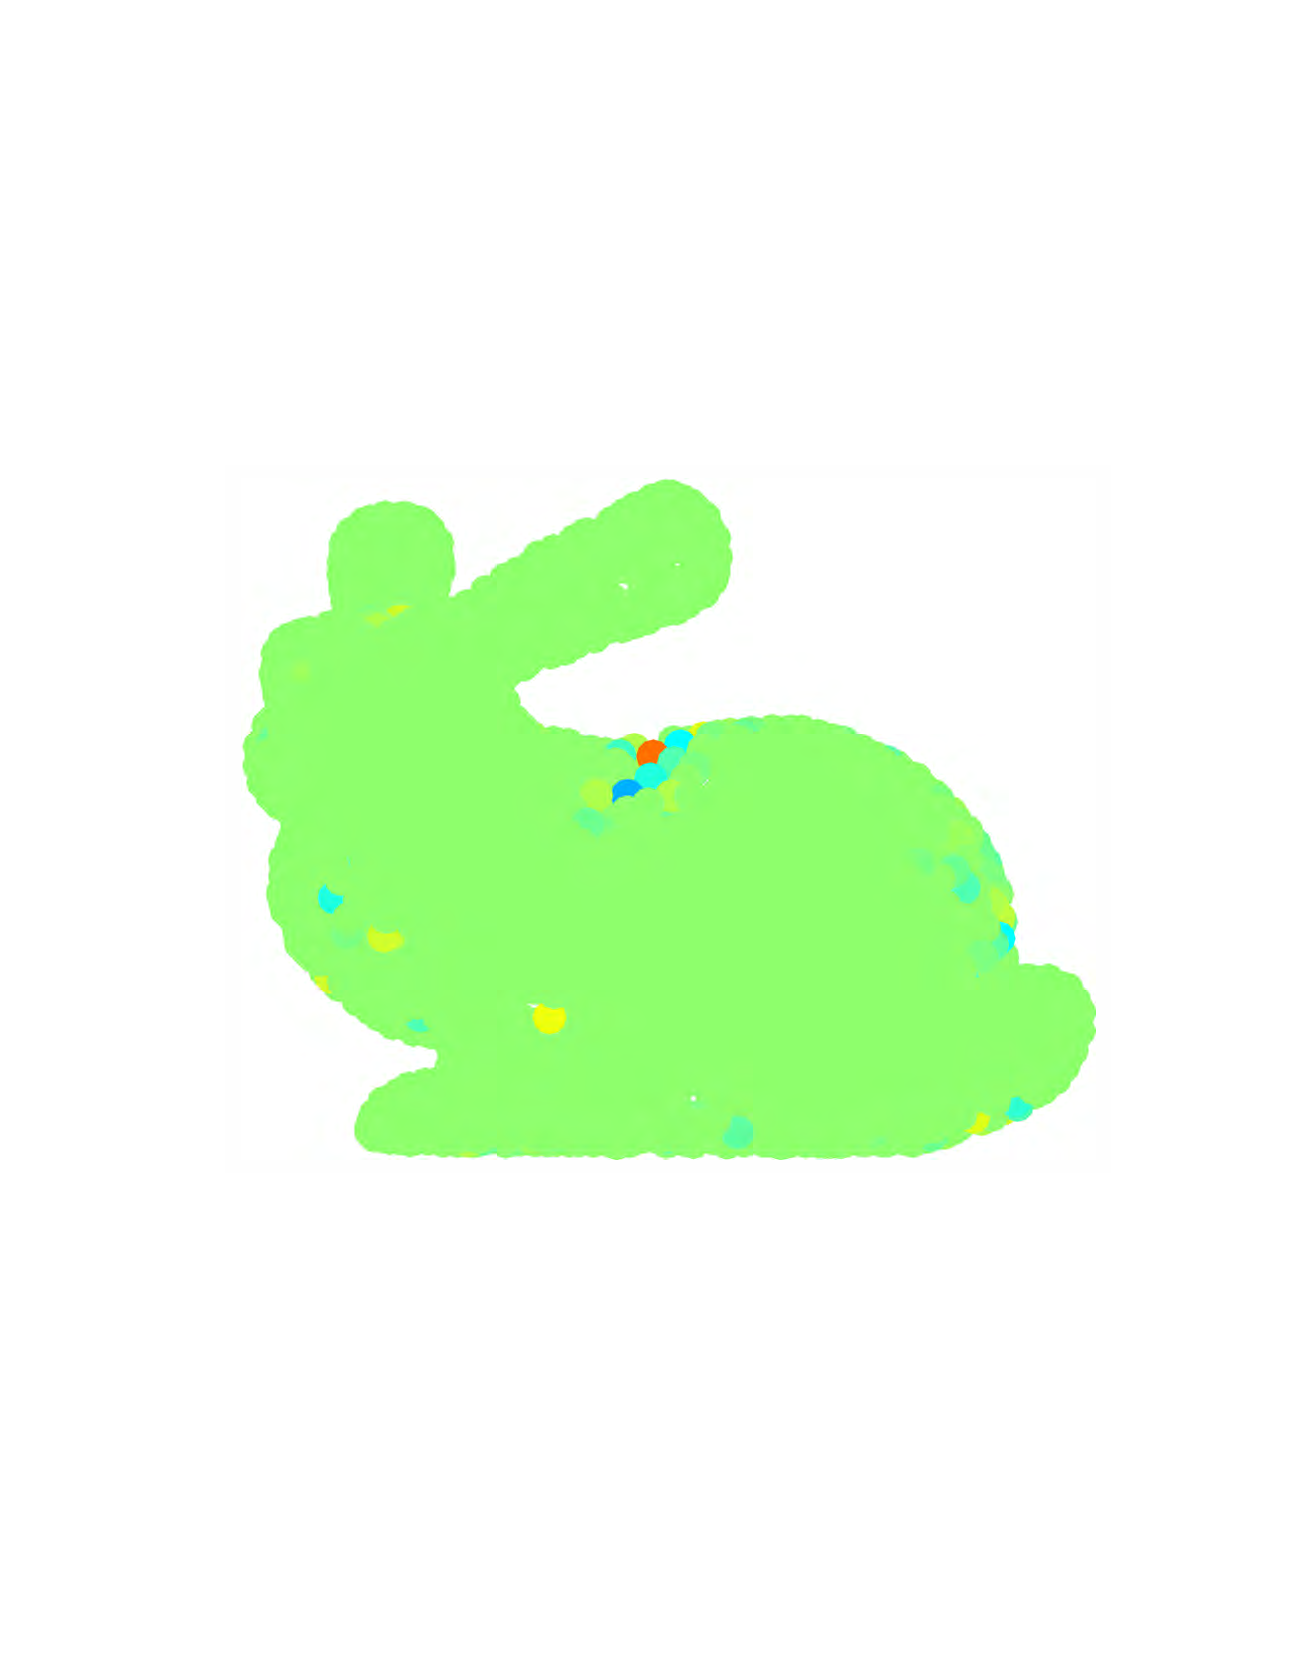
\includegraphics[width=.8\linewidth]{fig_bunny_coef_wav1}}
\end{minipage}
\begin{minipage}[m]{0.16\linewidth}
\centerline{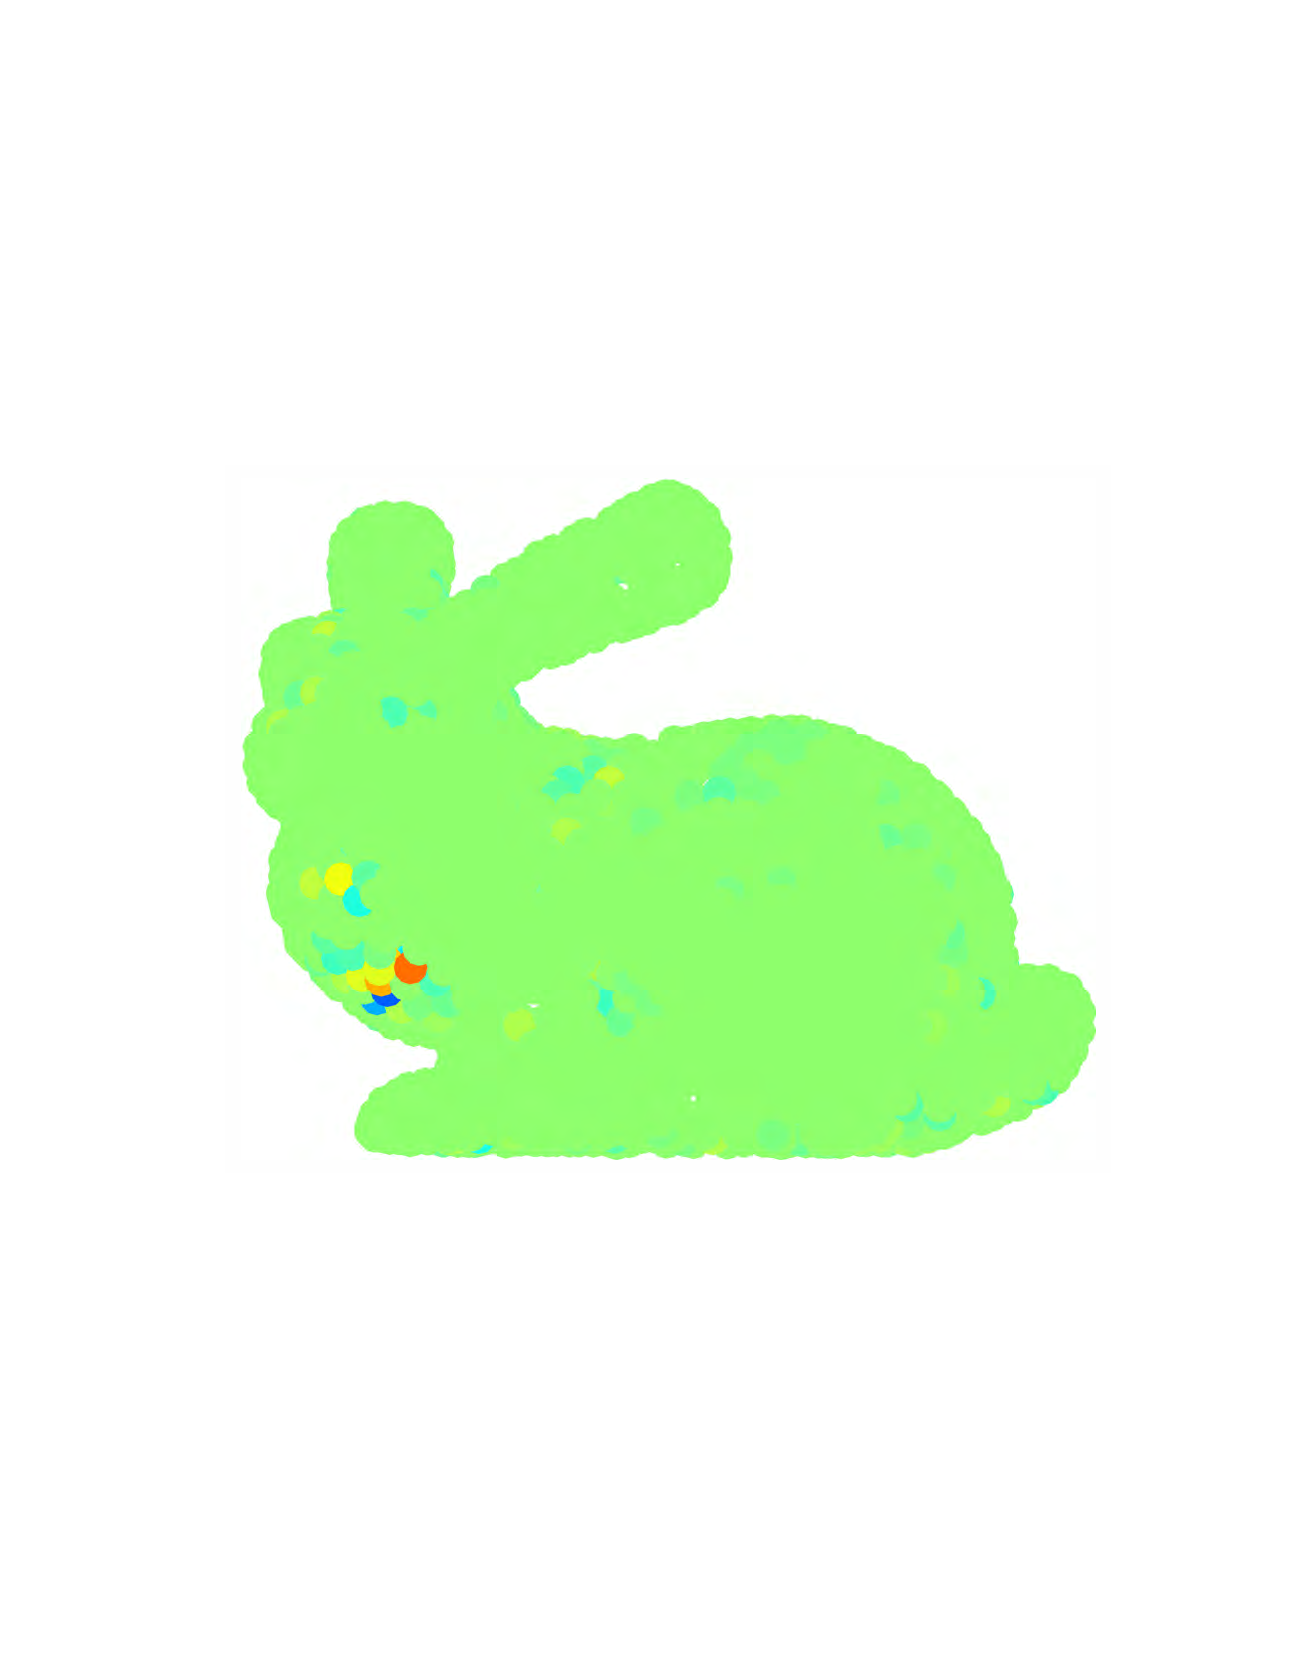
\includegraphics[width=.8\linewidth]{fig_bunny_coef_wav2}}
\end{minipage}
\begin{minipage}[m]{0.16\linewidth}
\centerline{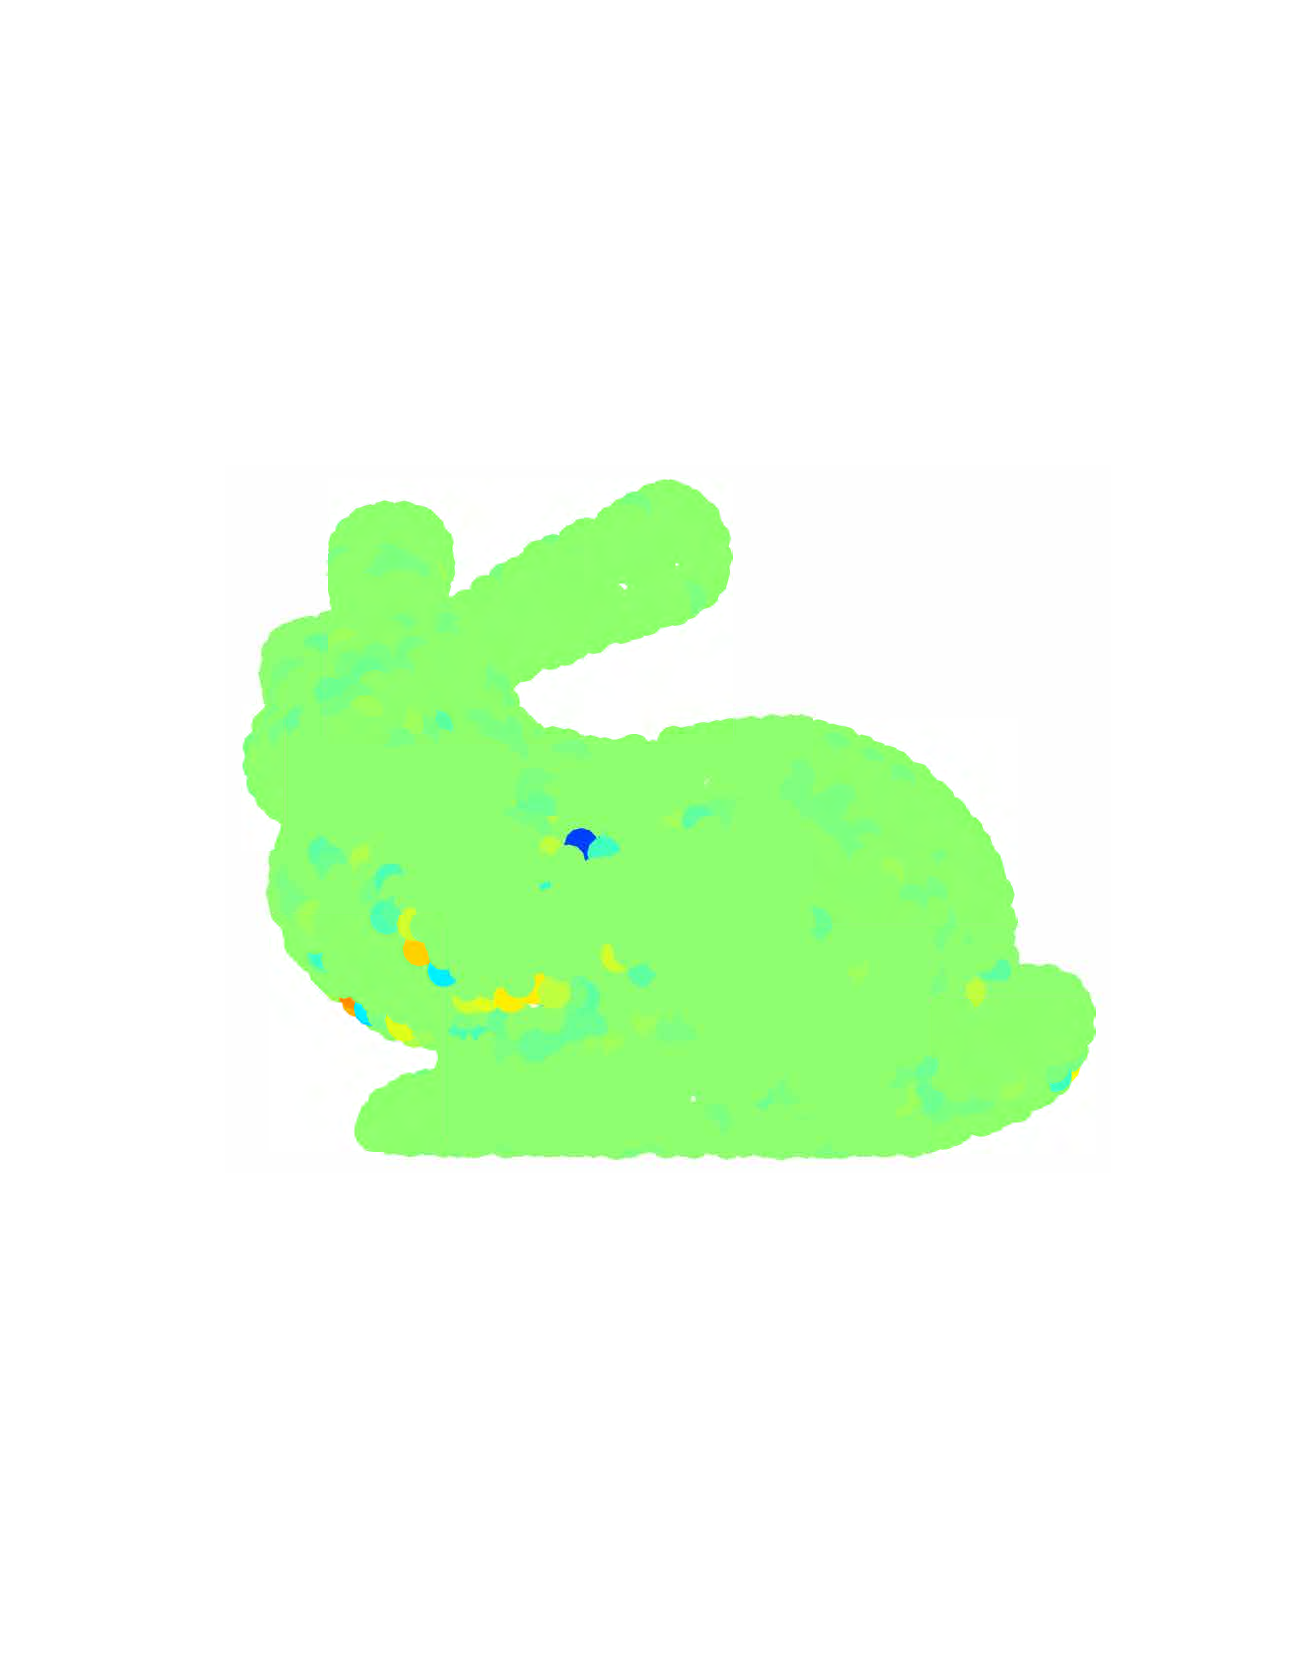
\includegraphics[width=.8\linewidth]{fig_bunny_coef_wav3}}
\end{minipage}
\begin{minipage}[m]{0.16\linewidth}
\centerline{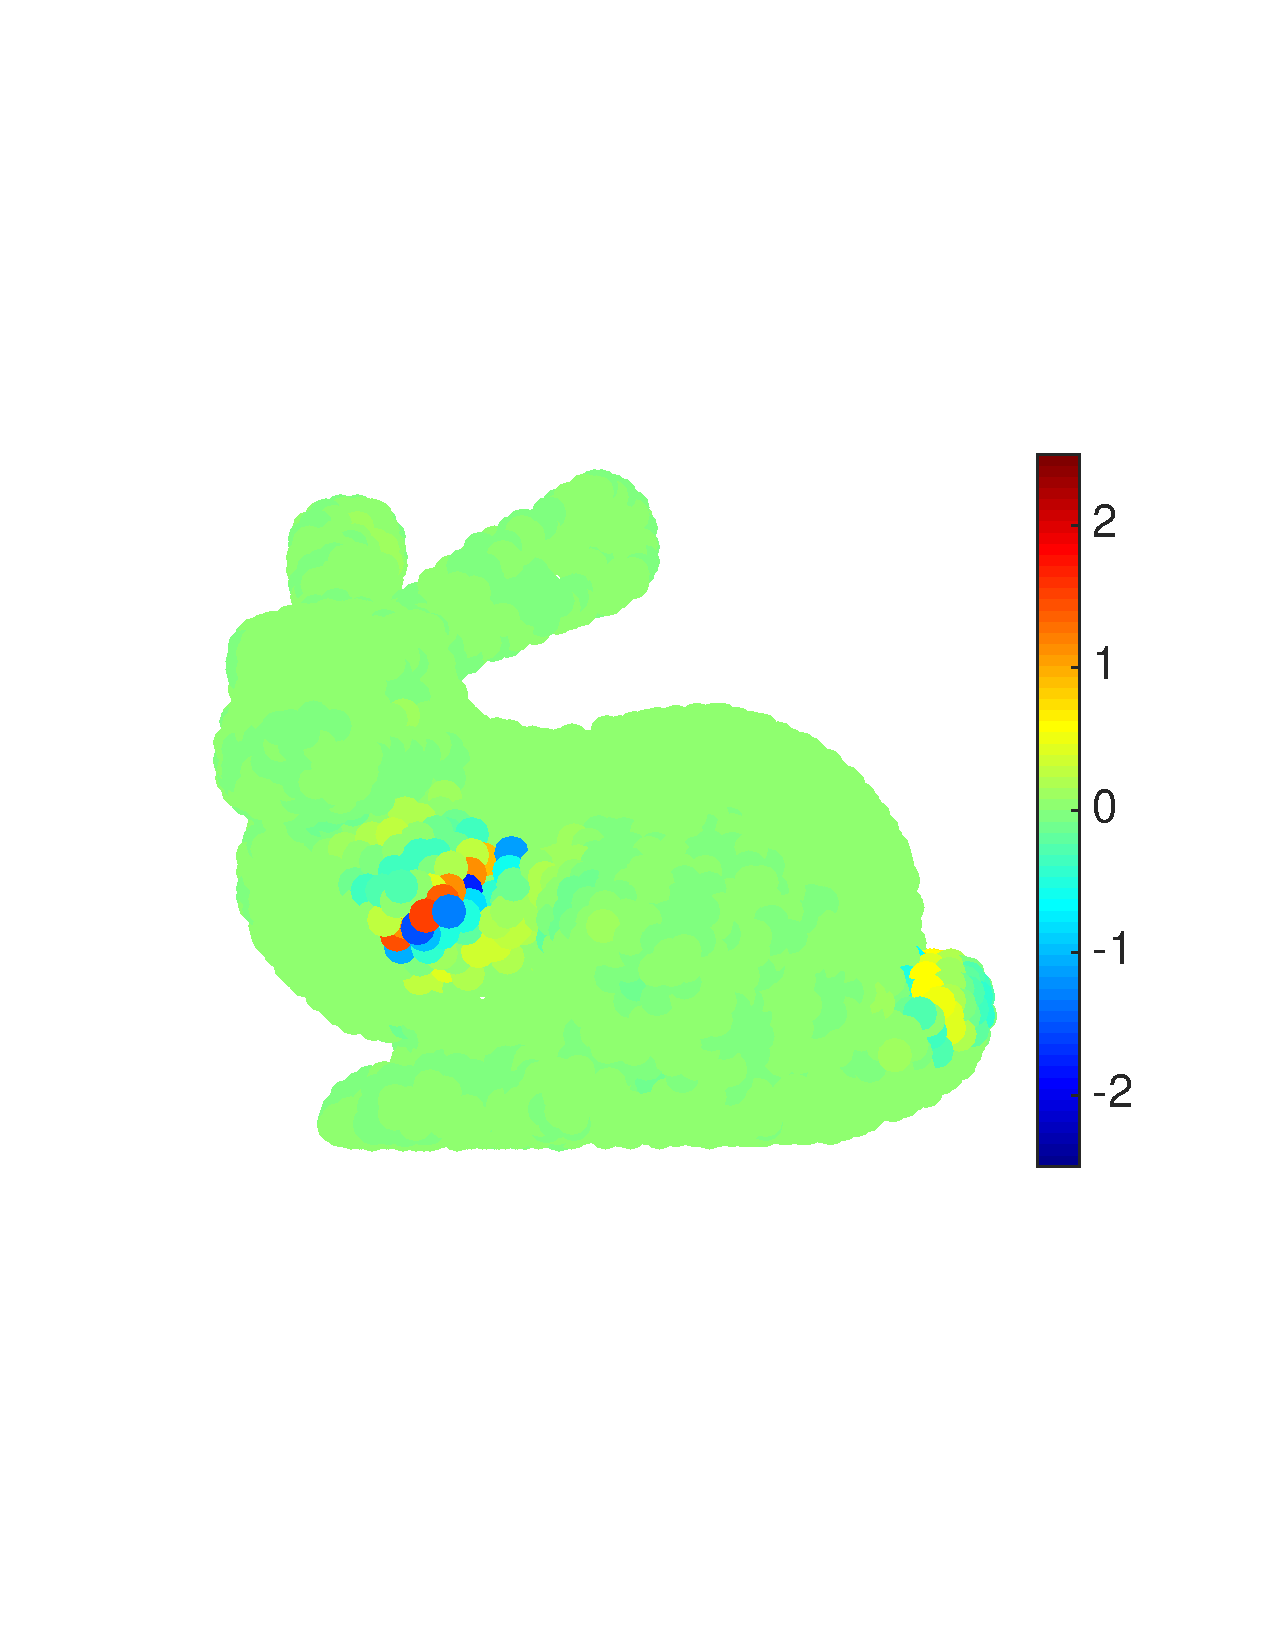
\includegraphics[width=.85\linewidth]{fig_bunny_coef_wav4}}
\end{minipage}\\
\begin{minipage}[m]{0.16\linewidth}
\centerline{\small{Reconstruction}}
\centerline{\small{by Band}}
\end{minipage}
\begin{minipage}[m]{0.16\linewidth}
\centerline{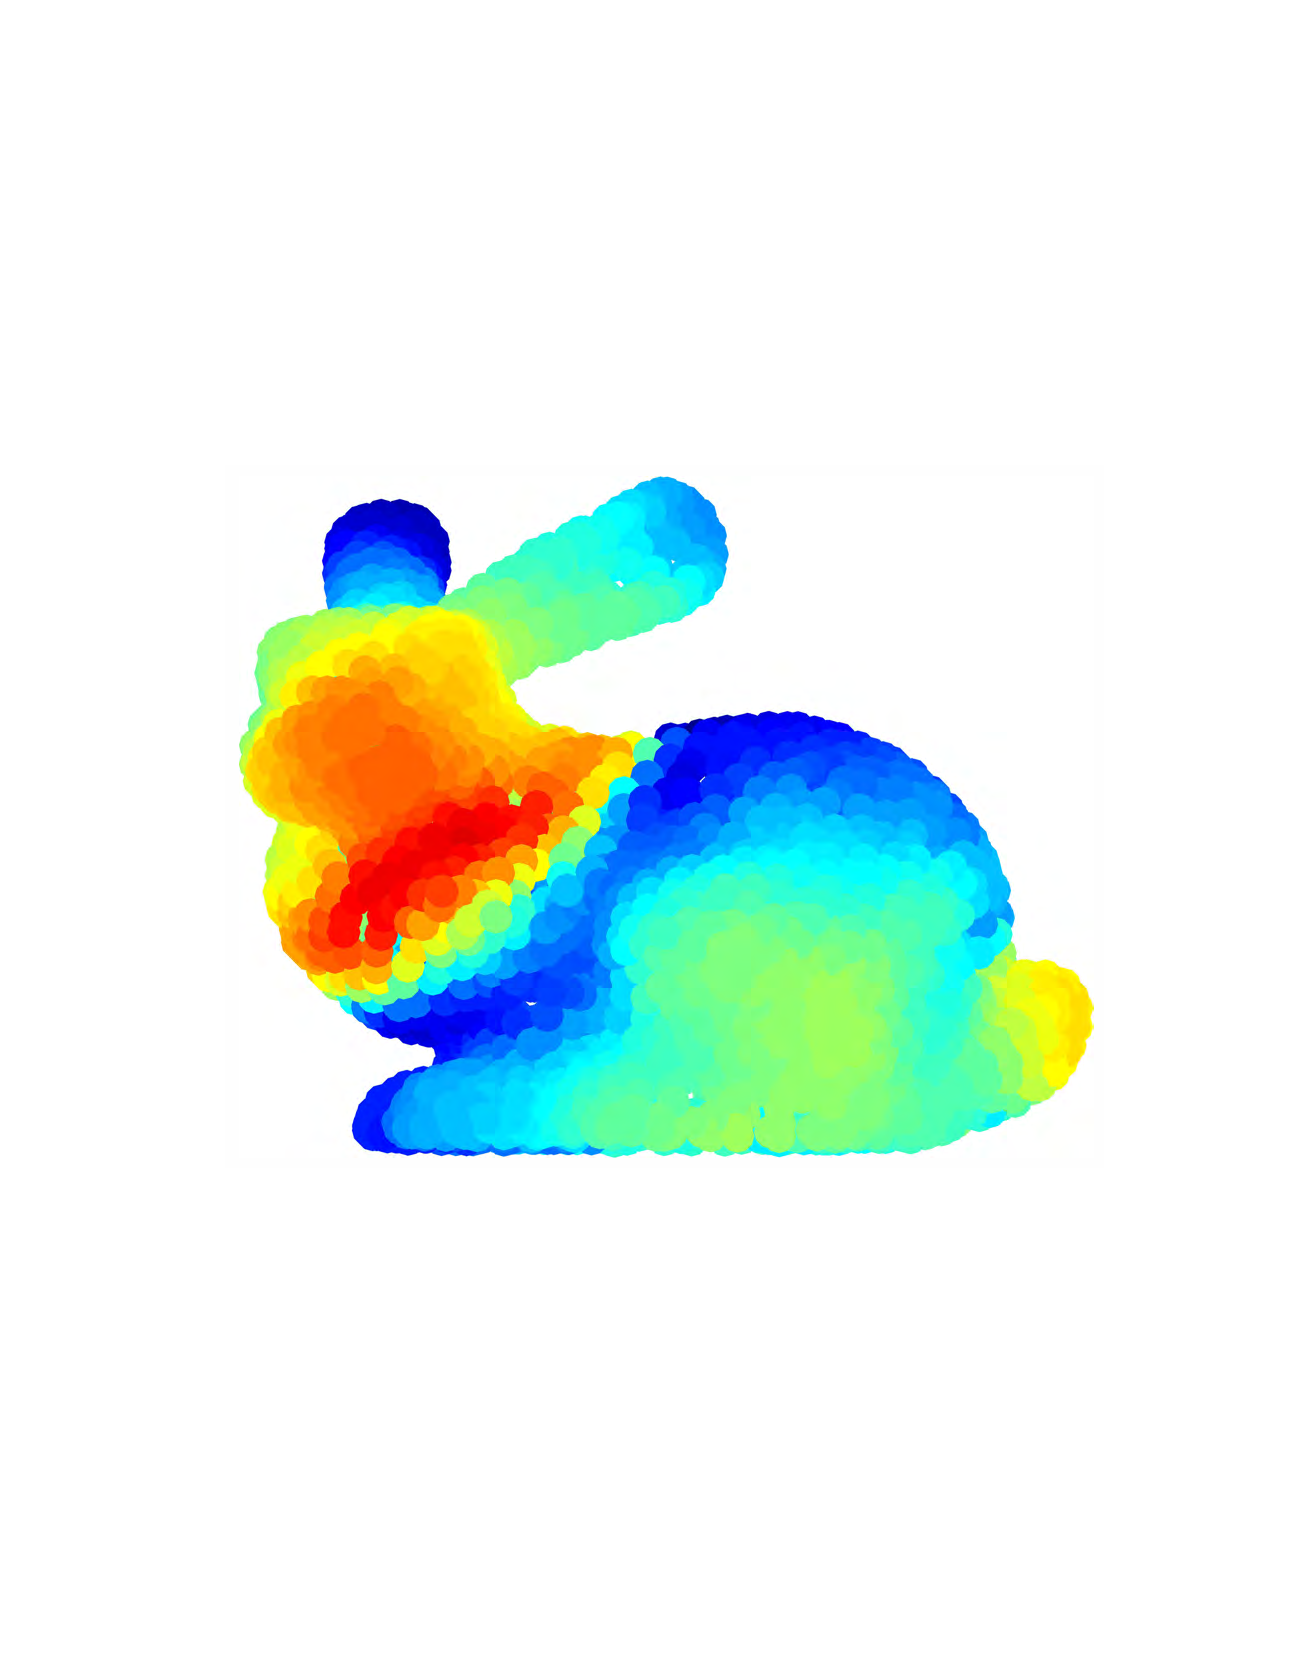
\includegraphics[width=.8\linewidth]{fig_bunny_rec_scaling}}
\end{minipage}
\begin{minipage}[m]{0.16\linewidth}
\centerline{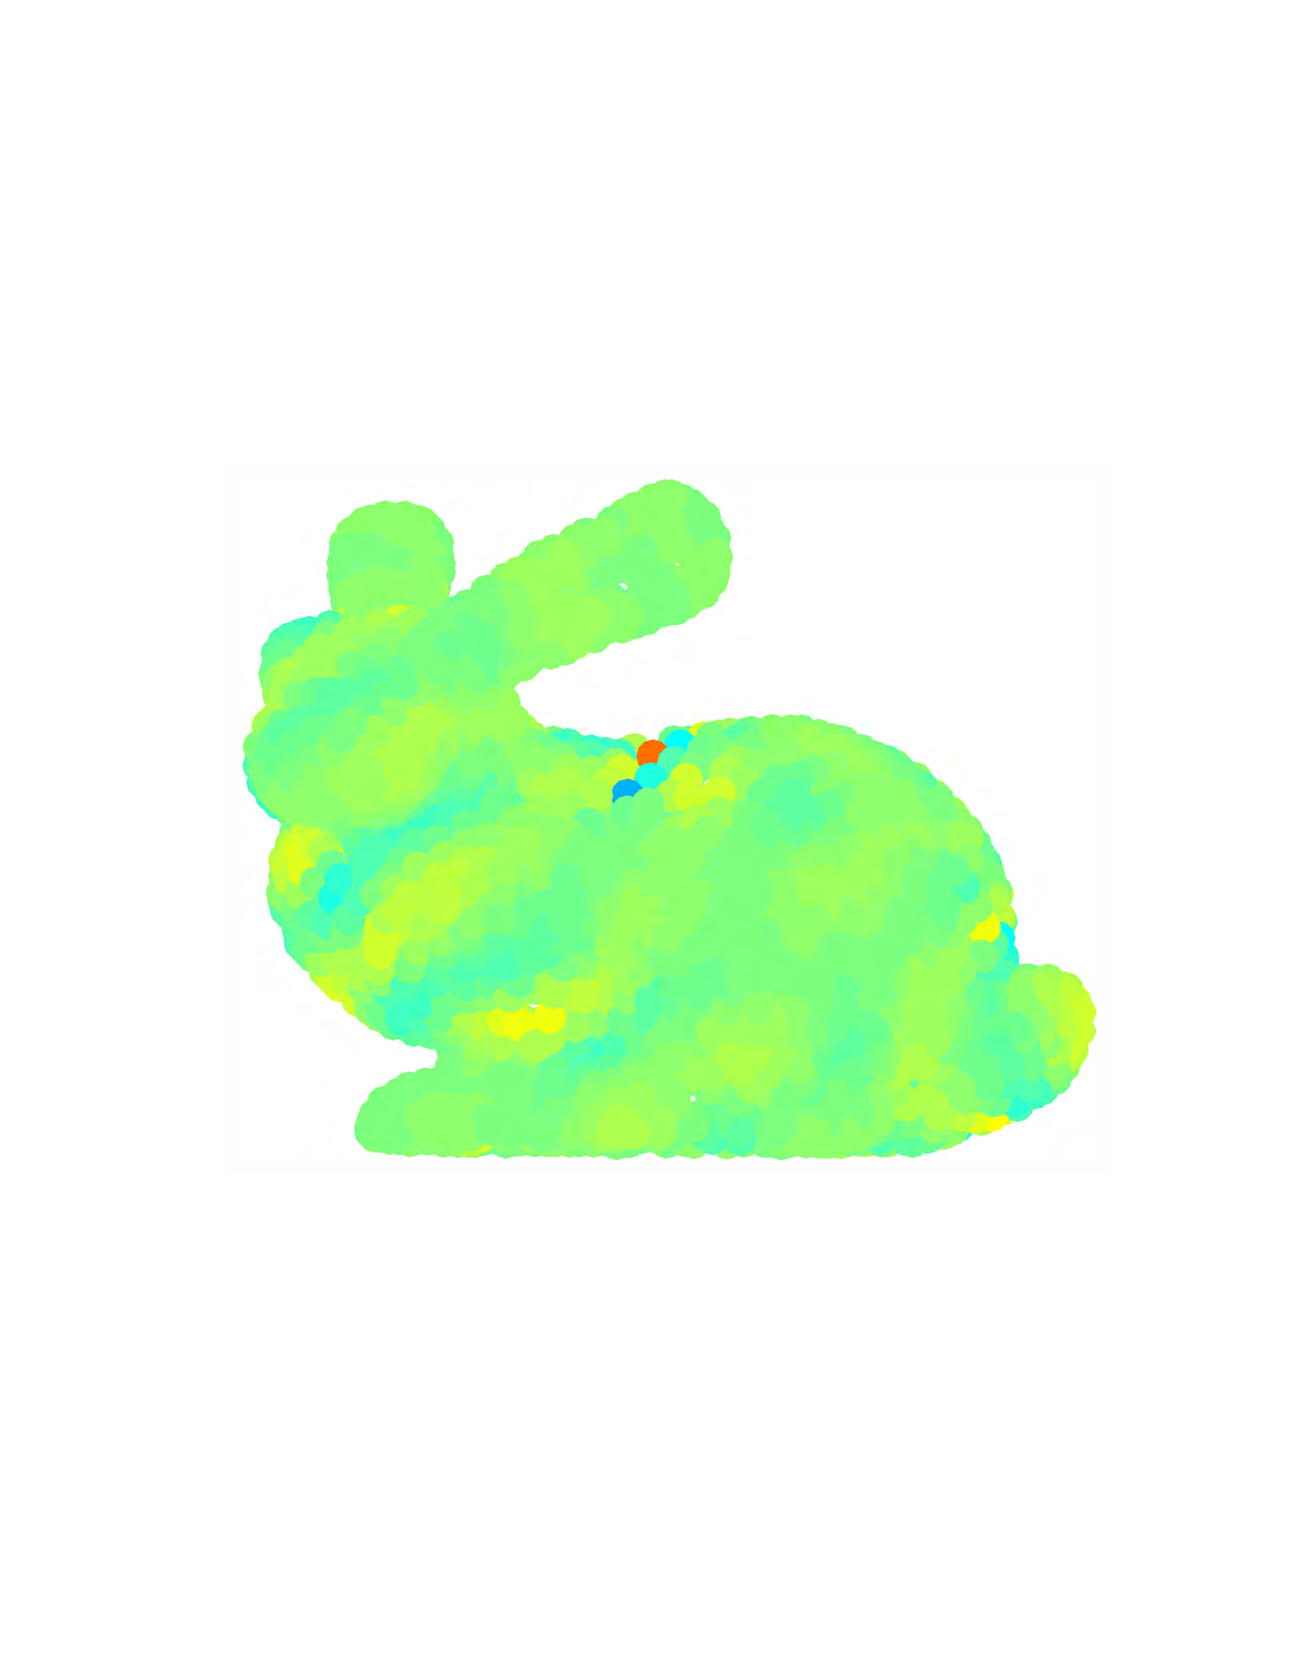
\includegraphics[width=.8\linewidth]{fig_bunny_rec_wav1}}
\end{minipage}
\begin{minipage}[m]{0.16\linewidth}
\centerline{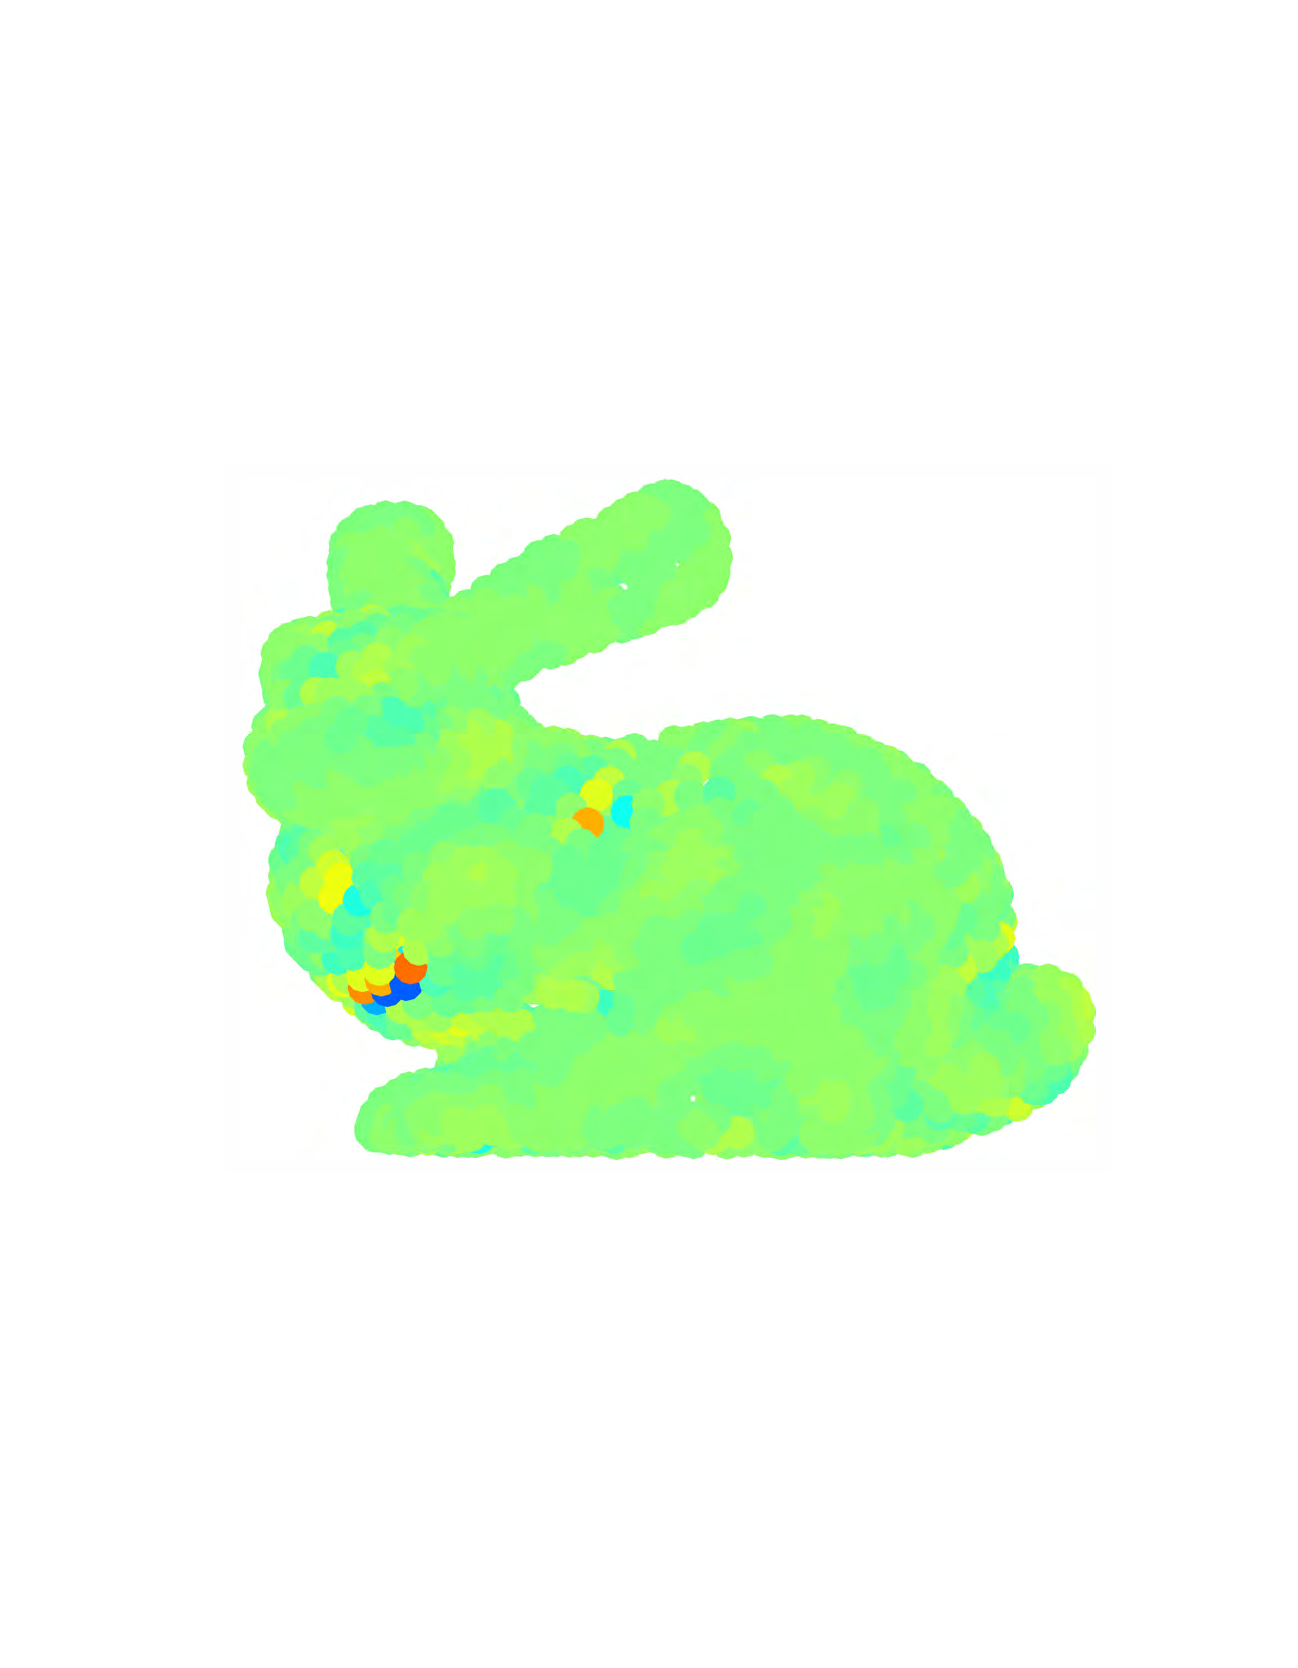
\includegraphics[width=.8\linewidth]{fig_bunny_rec_wav2}}
\end{minipage}
\begin{minipage}[m]{0.16\linewidth}
\centerline{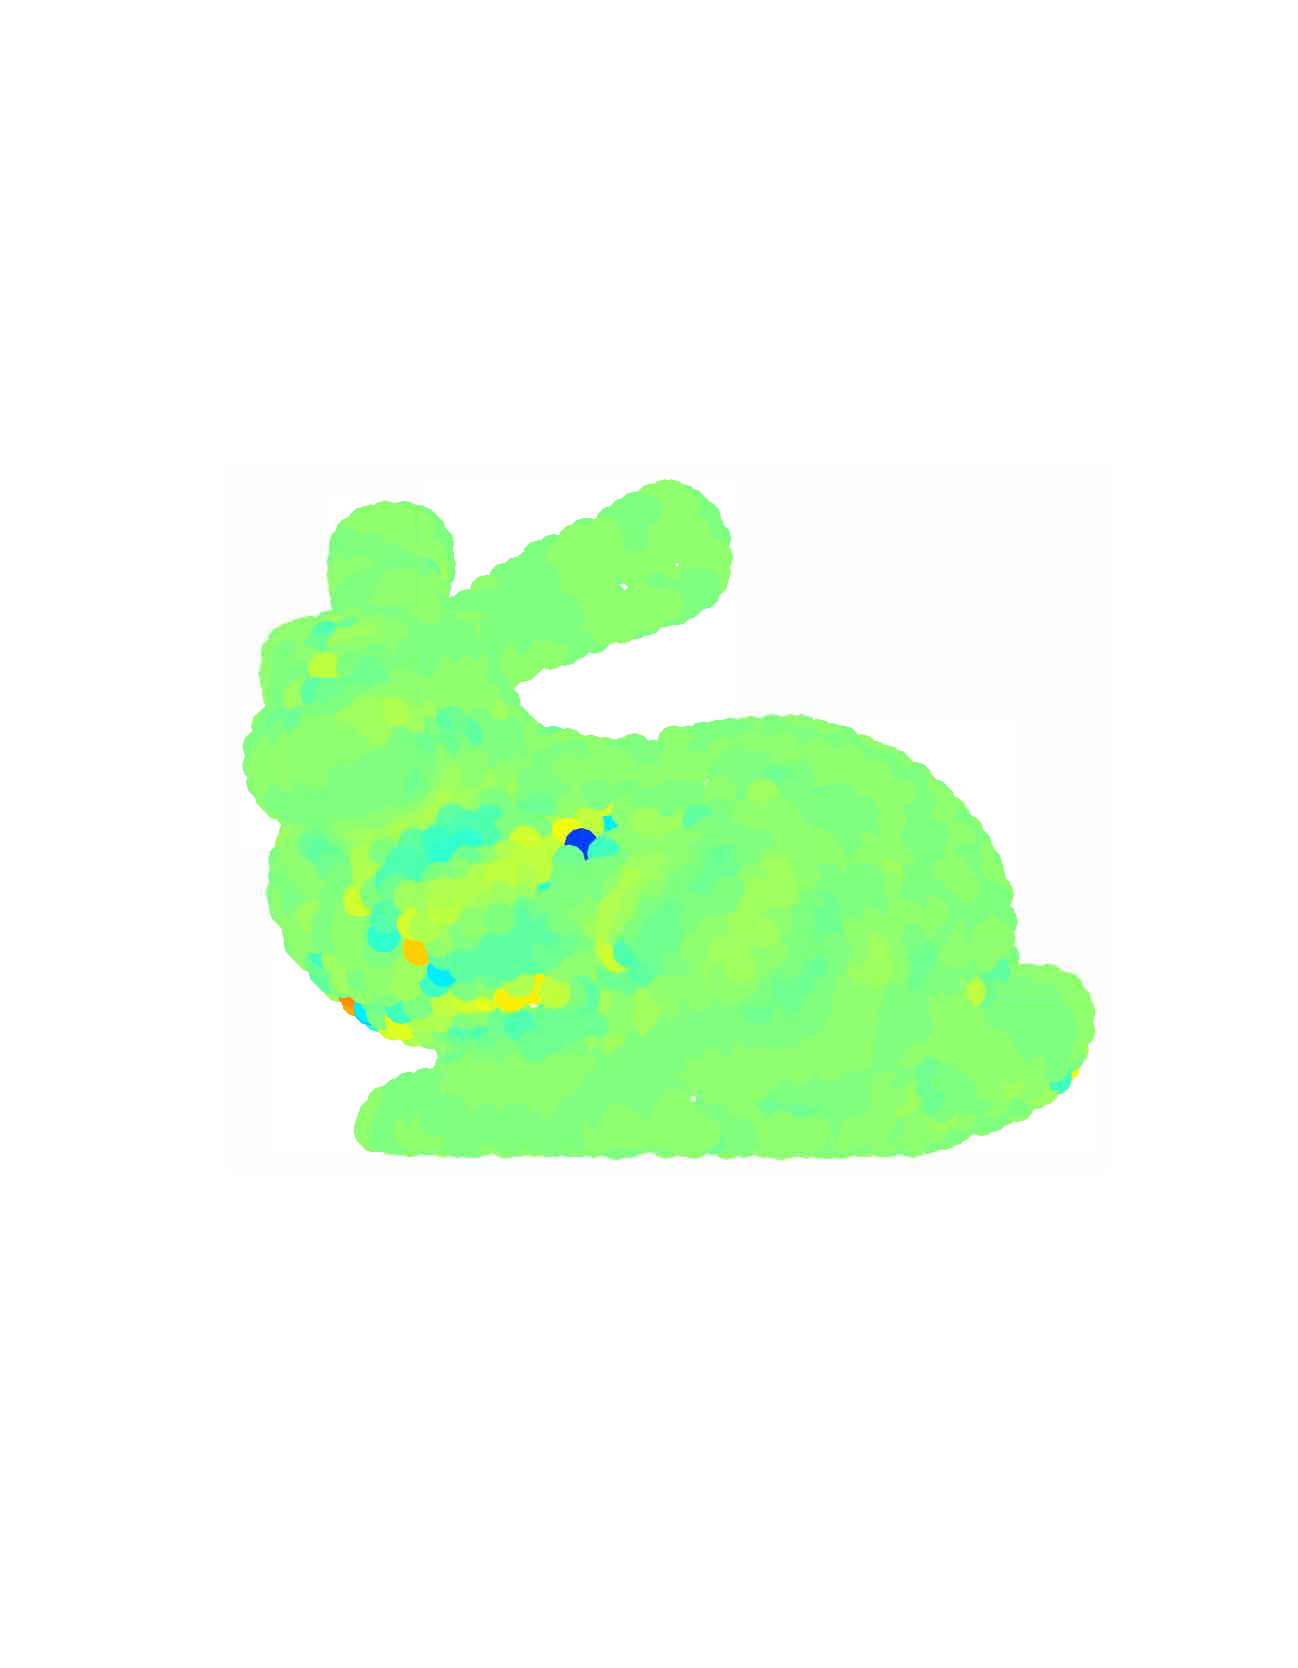
\includegraphics[width=.8\linewidth]{fig_bunny_rec_wav3}}
\end{minipage}
\begin{minipage}[m]{0.16\linewidth}
\centerline{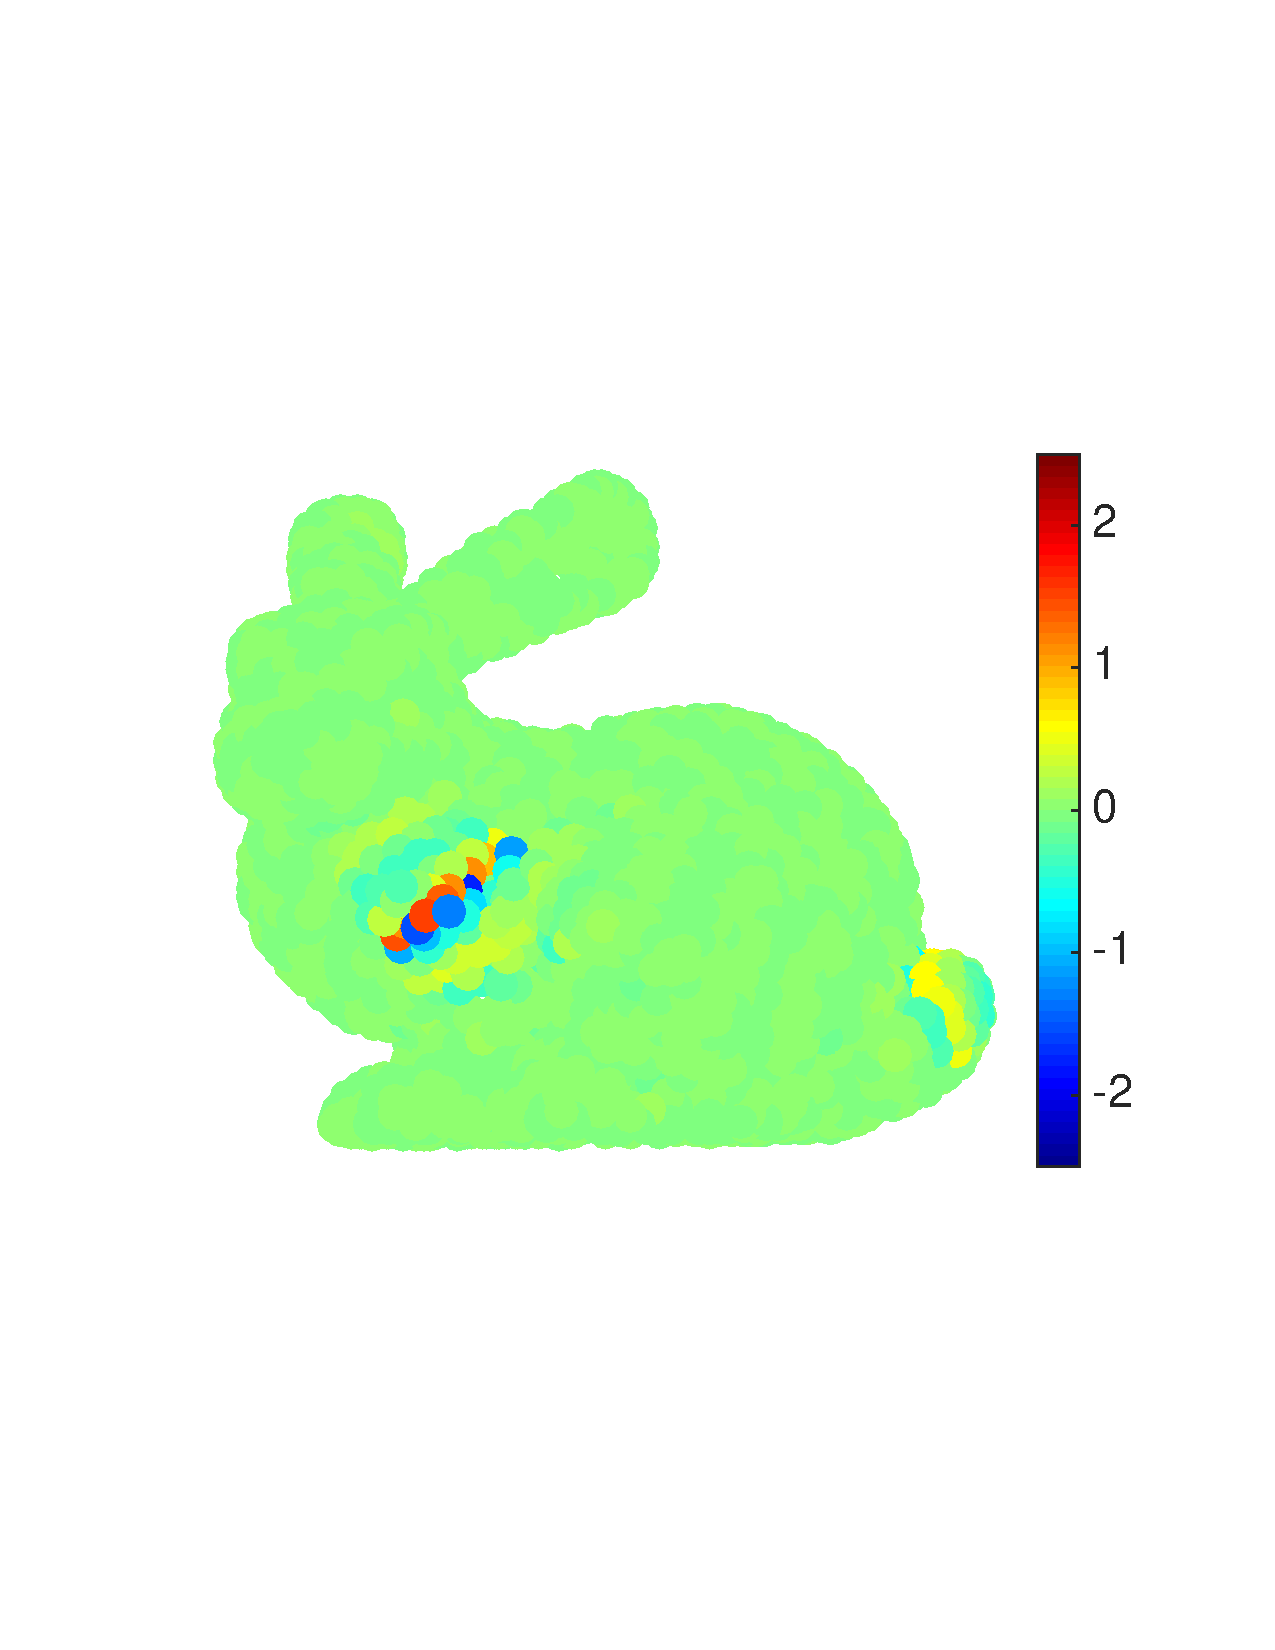
\includegraphics[width=.85\linewidth]{fig_bunny_rec_wav4}}
\end{minipage}
\caption{$M$-channel filter bank example. The first row shows example atoms in the vertex domain. The second row shows all atoms in the spectral domain, with an average of the atoms in each band shown by the thick black lines. The third row shows the analysis coefficients of Fig.\ \ref{Fig:bunny_signal}(d) by band, and the last row is the interpolation by band from those coefficients.}\label{Fig:bunny_coef}
\end{figure*}

\begin{figure}[tbh]
\begin{minipage}[m]{0.48\linewidth}
\centerline{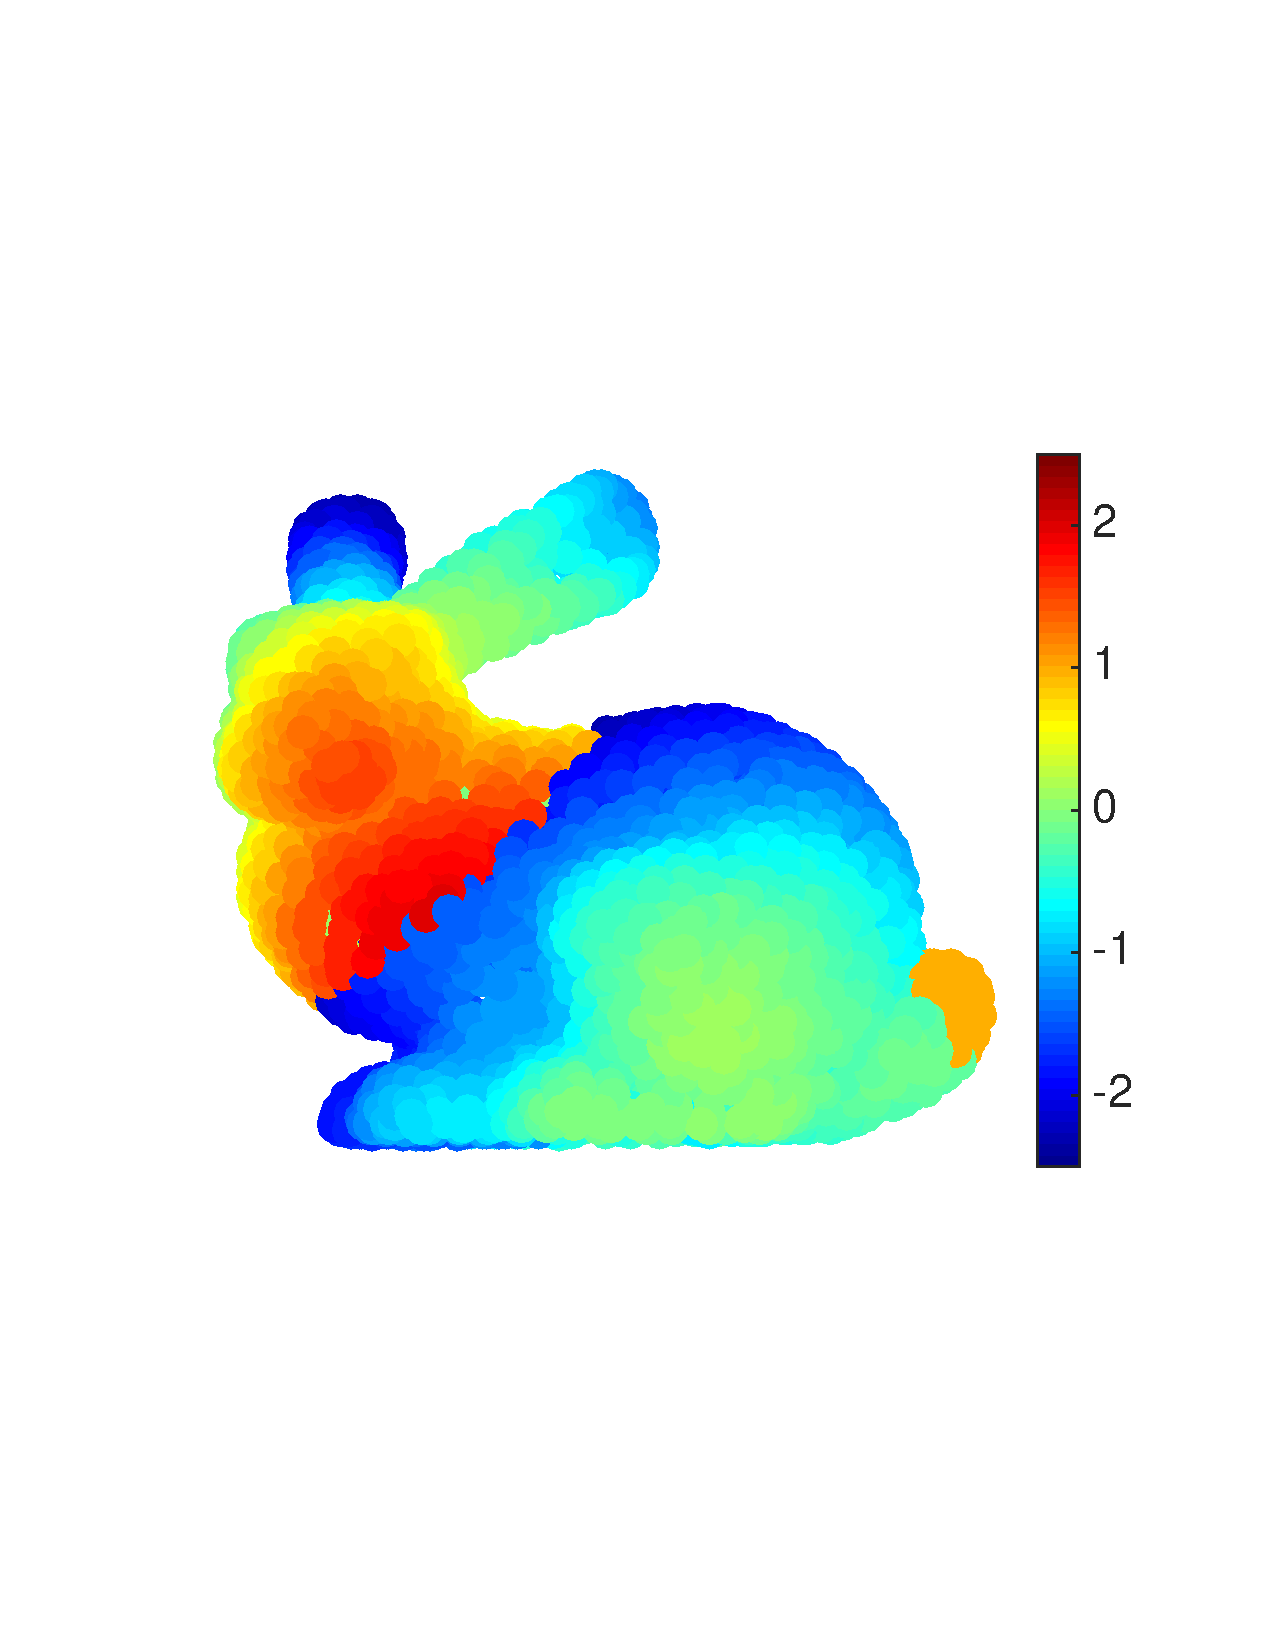
\includegraphics[width=.8\linewidth]{fig_bunny_signal}}
\centerline{\small{(a)}}
\end{minipage}
\begin{minipage}[m]{0.48\linewidth}
\centerline{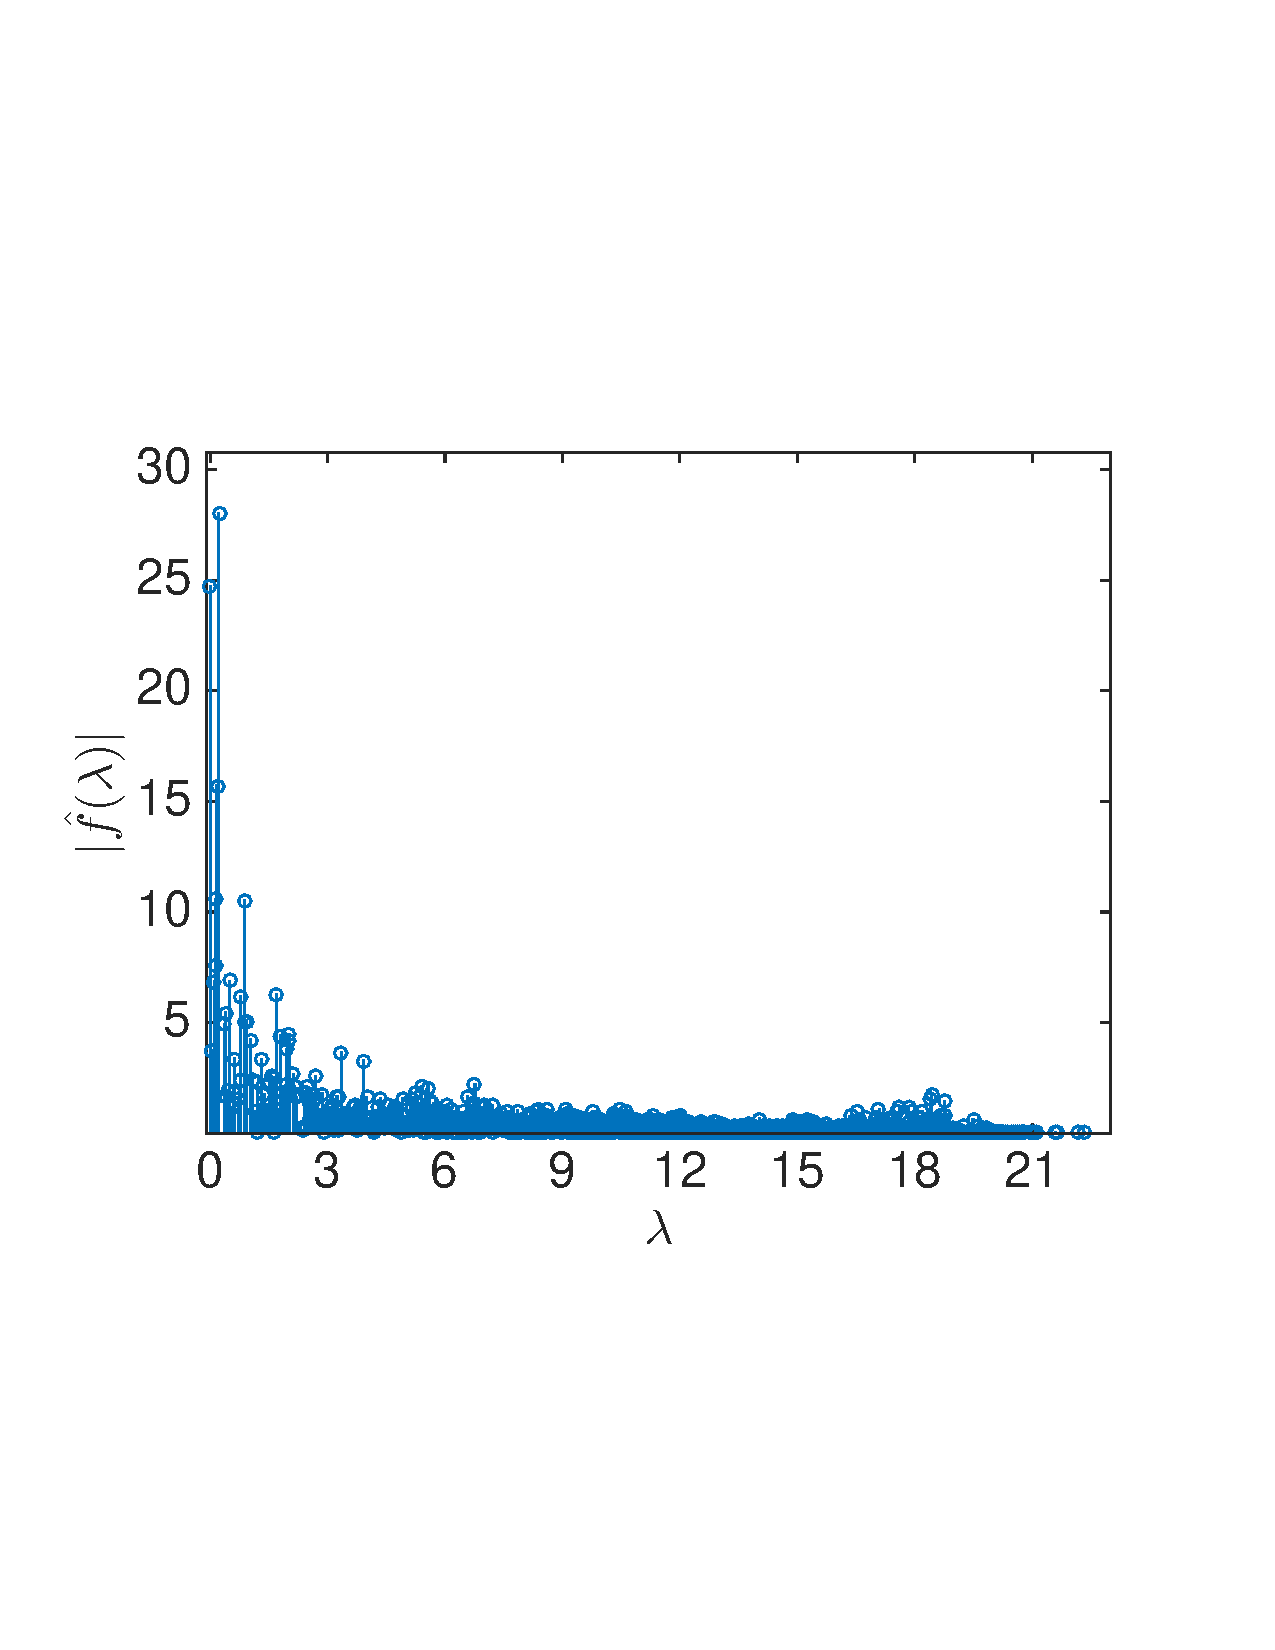
\includegraphics[width=.8\linewidth]{fig_bunny_signal_hat}~~~~~~~}
\centerline{\small{(b)}}
\end{minipage} \\
\begin{minipage}[m]{0.48\linewidth}
\centerline{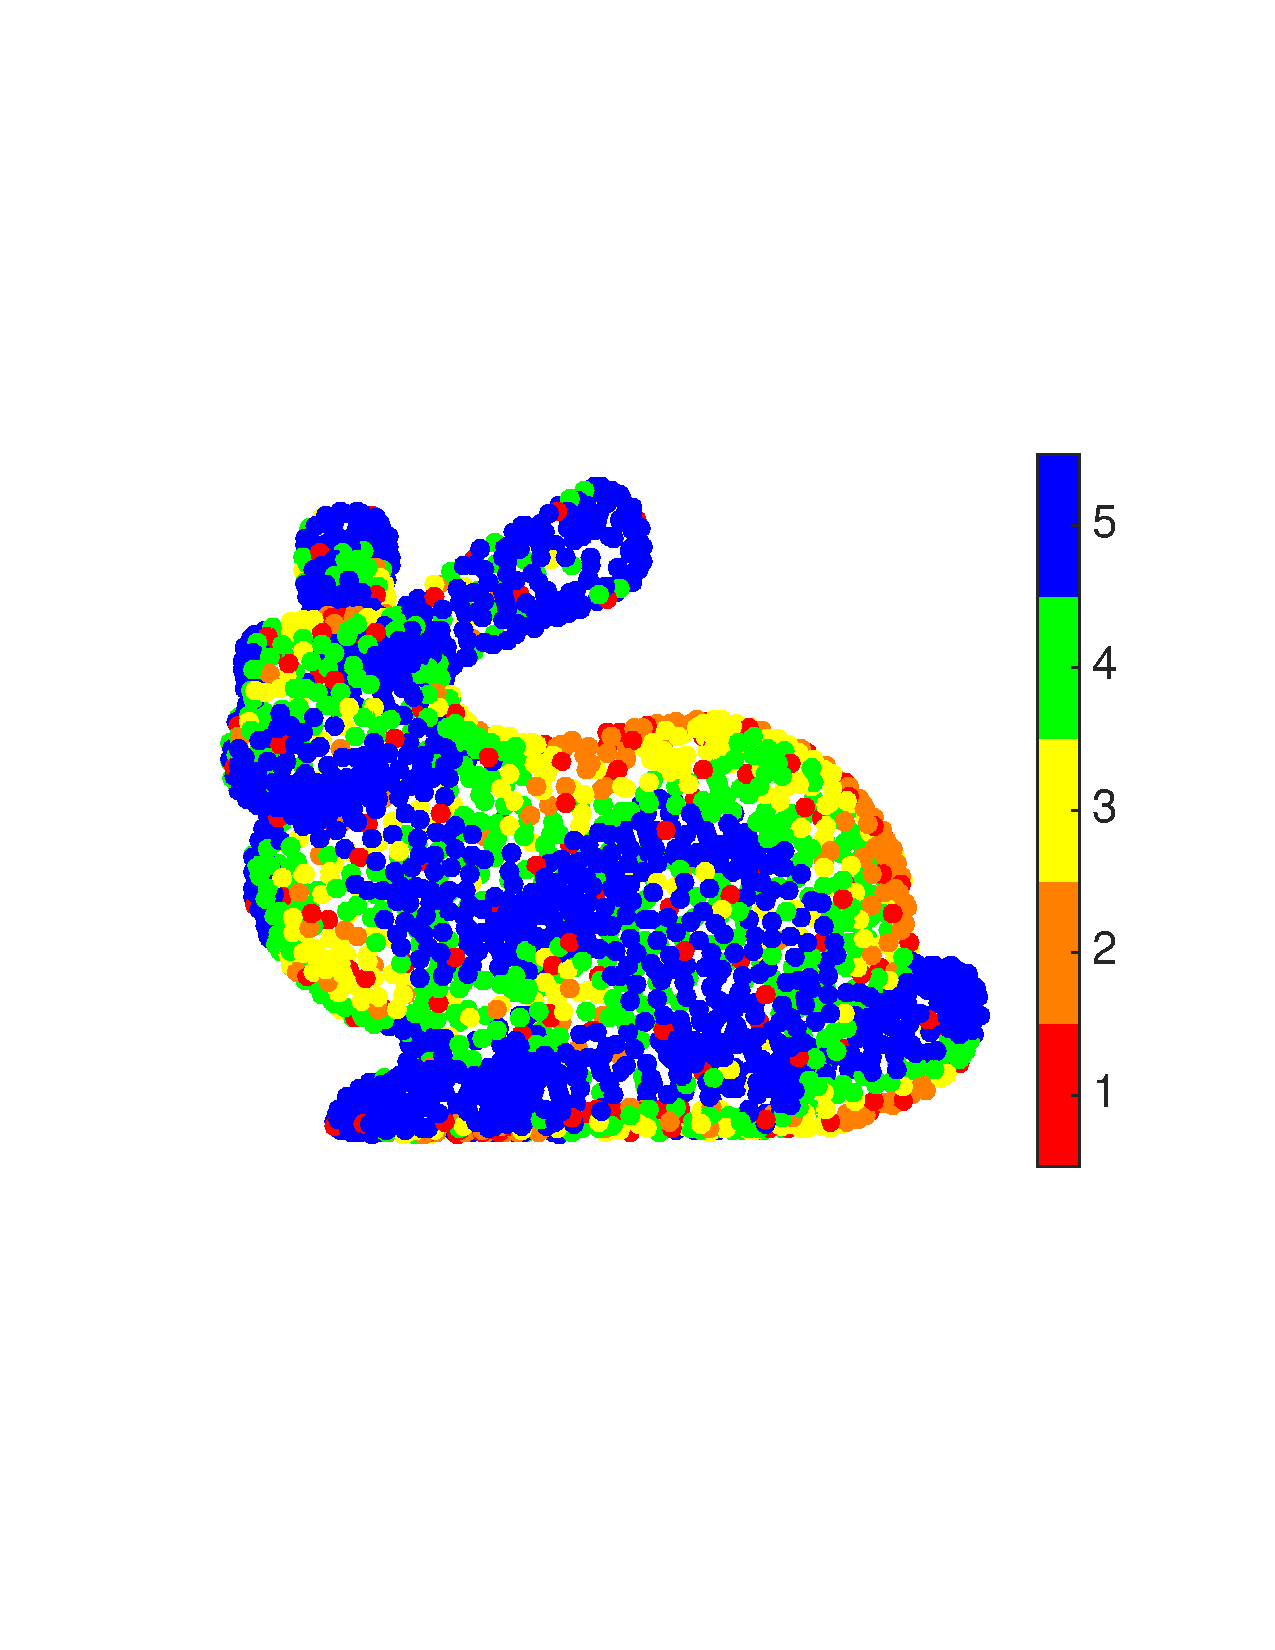
\includegraphics[width=.8\linewidth]{fig_bunny_partition}}
\centerline{\small{(c)}}
\end{minipage}
\begin{minipage}[m]{0.48\linewidth}
\centerline{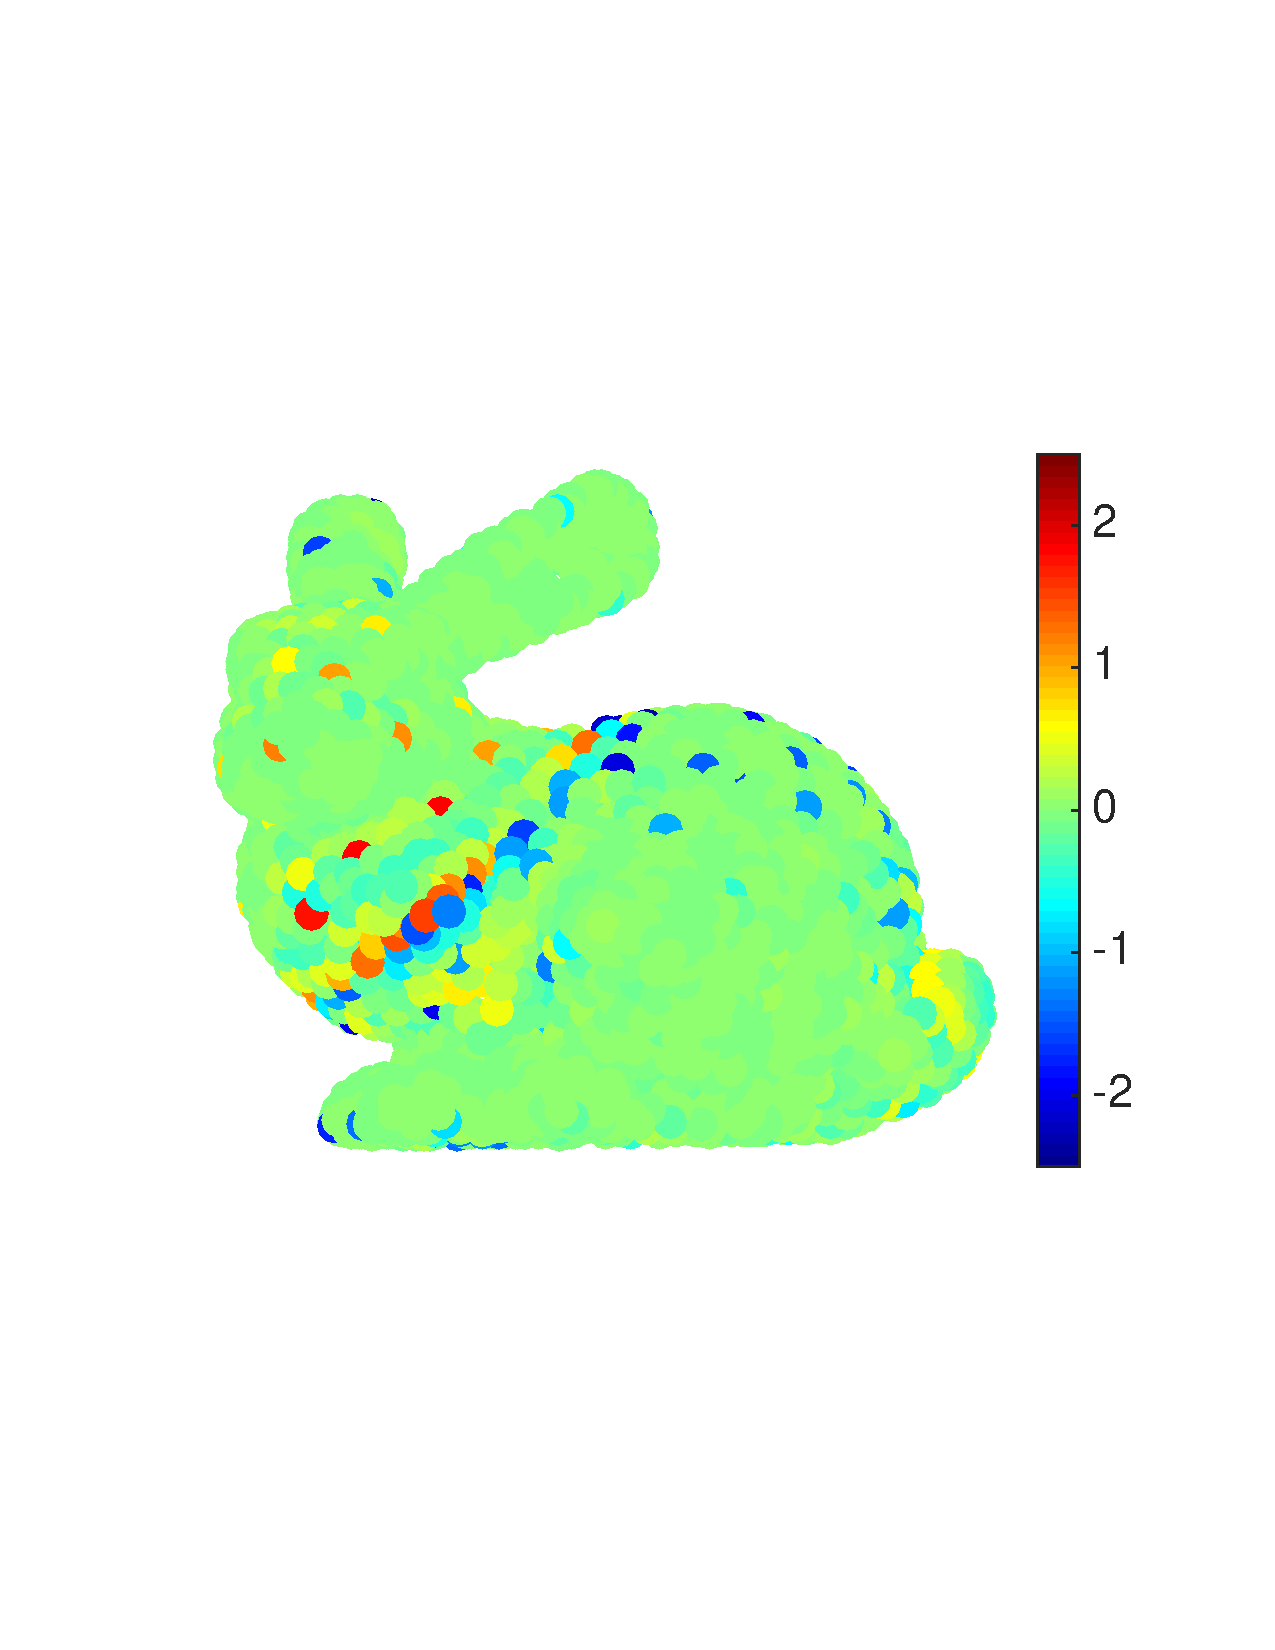
\includegraphics[width=.8\linewidth]{fig_bunny_coef_all}}
\centerline{\small{(d)}}
\end{minipage}
\caption{(a)-(b) Piecewise smooth signal on the Stanford bunny graph \cite{bunny} in the vertex and graph spectral domains, respectively. (c) Partition of the graph into uniqueness sets for five different spectral bands. (d) $M$-channel filter bank analysis coefficients of the signal shown in (a) and (b).}\label{Fig:bunny_signal}
\end{figure}

\subsection{Joint vertex-frequency localization of atoms and example analysis coefficients}
We start by empirically showing that the dictionary atoms (the columns of $\boldsymbol{\Phi}$) are jointly localized in the vertex and graph spectral domains. On the Stanford bunny graph \cite{bunny} with 2503 vertices, we partition the spectrum into five bands, and show the resulting partition into uniqueness sets 
in Fig.\ \ref{Fig:bunny_signal}(c). The first row of Fig.\ \ref{Fig:bunny_coef} shows five different example atoms whose energy is concentrated on different spectral bands. We see that these atoms are generally localized in the vertex domain as well. Some atoms such as the one shown at wavelet scale 3 are more spread in the vertex domain, possibly as a result of using ideal filters in the filter bank, an issue we revisit in Section \ref{Se:filtering}. The second row of Fig.\ \ref{Fig:bunny_coef} shows the spectral content of all atoms in each band, with the average for each represented by a thick black line. As expected, the energies of the atoms are localized in the spectral domain as well. While the transform is not orthogonal, each atom is orthogonal to all atoms concentrated on other spectral bands. One possible extension is to find a fast algorithm to orthogonalize the atoms within each band. Note also that the wavelet atoms at all scales have mean zero, as they have no energy at eigenvalue zero.

Next we apply the proposed transform to a piecewise-smooth graph signal $f$ that is shown in the vertex domain in Fig.\ \ref{Fig:bunny_signal}(a), and in the graph spectral domain in Fig.\ \ref{Fig:bunny_signal}(b). The full set of analysis coefficients is shown in Fig.\ \ref{Fig:bunny_signal}(d), and these are separated by band in the third row of Fig.\ \ref{Fig:bunny_coef}. We see that with the exception of the lowpass channel, the coefficients are clustered around the two main discontinuities (around the midsection and tail of the bunny). The bottom row of Fig.\ \ref{Fig:bunny_coef} shows the interpolation of these coefficients onto the corresponding spectral bands, and if we sum these reconstructions together, we recover exactly the original signal in Fig.\ \ref{Fig:bunny_signal}(a).


\subsection{Sparse approximation}
Next, we compress 
a piecewise-smooth graph signal $f$ via the sparse coding optimization
\begin{align}\label{Eq:sparse_coding}
\argmin_x   || f-\boldsymbol{\Phi}x ||_2^2 \hbox{~~~subject to } ||x||_0 \leq T,
\end{align}
where $T$ is a predefined sparsity level. After first normalizing the atoms of various critically-sampled dictionaries, we use the greedy %approximately solve the optimization problem
 % with 
 orthogonal matching pursuit (OMP) algorithm \cite{tropp2004greed,elad_book} to approximately solve \eqref{Eq:sparse_coding}. For the $M$-channel filter bank, the partition into uniqueness sets is shown in Fig. \ref{Fig:part_examples}, and the filter bank is shown in Fig. \ref{Fig:fb}. We show the reconstruction errors in Fig. \ref{Fig:comp}(d). 

\begin{figure}[tbh]
\begin{minipage}[m]{0.48\linewidth}
\centerline{~~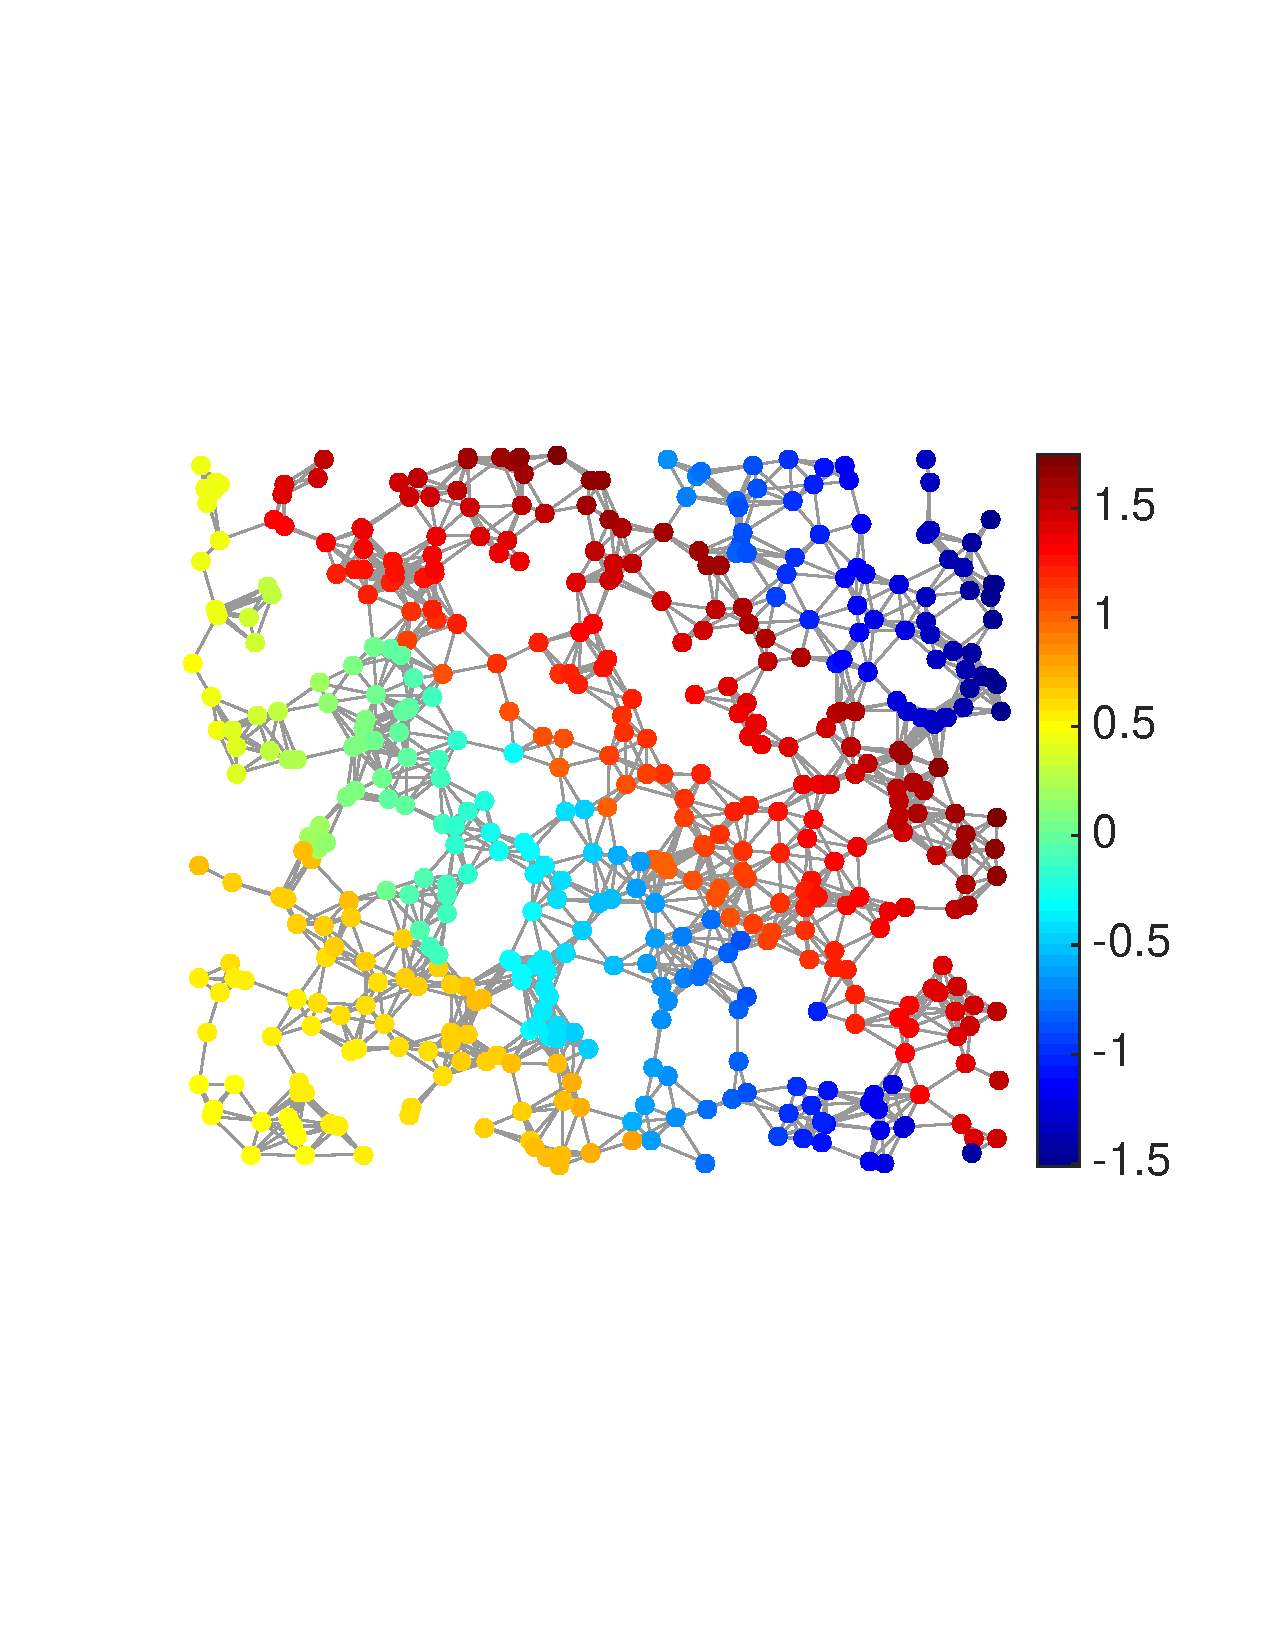
\includegraphics[width=.9\linewidth]{fig_comp_sig}}
\vspace{.05in}
\centerline{\small{(a)}}
\end{minipage}
\begin{minipage}[m]{0.48\linewidth}
\vspace{.02in}
\centerline{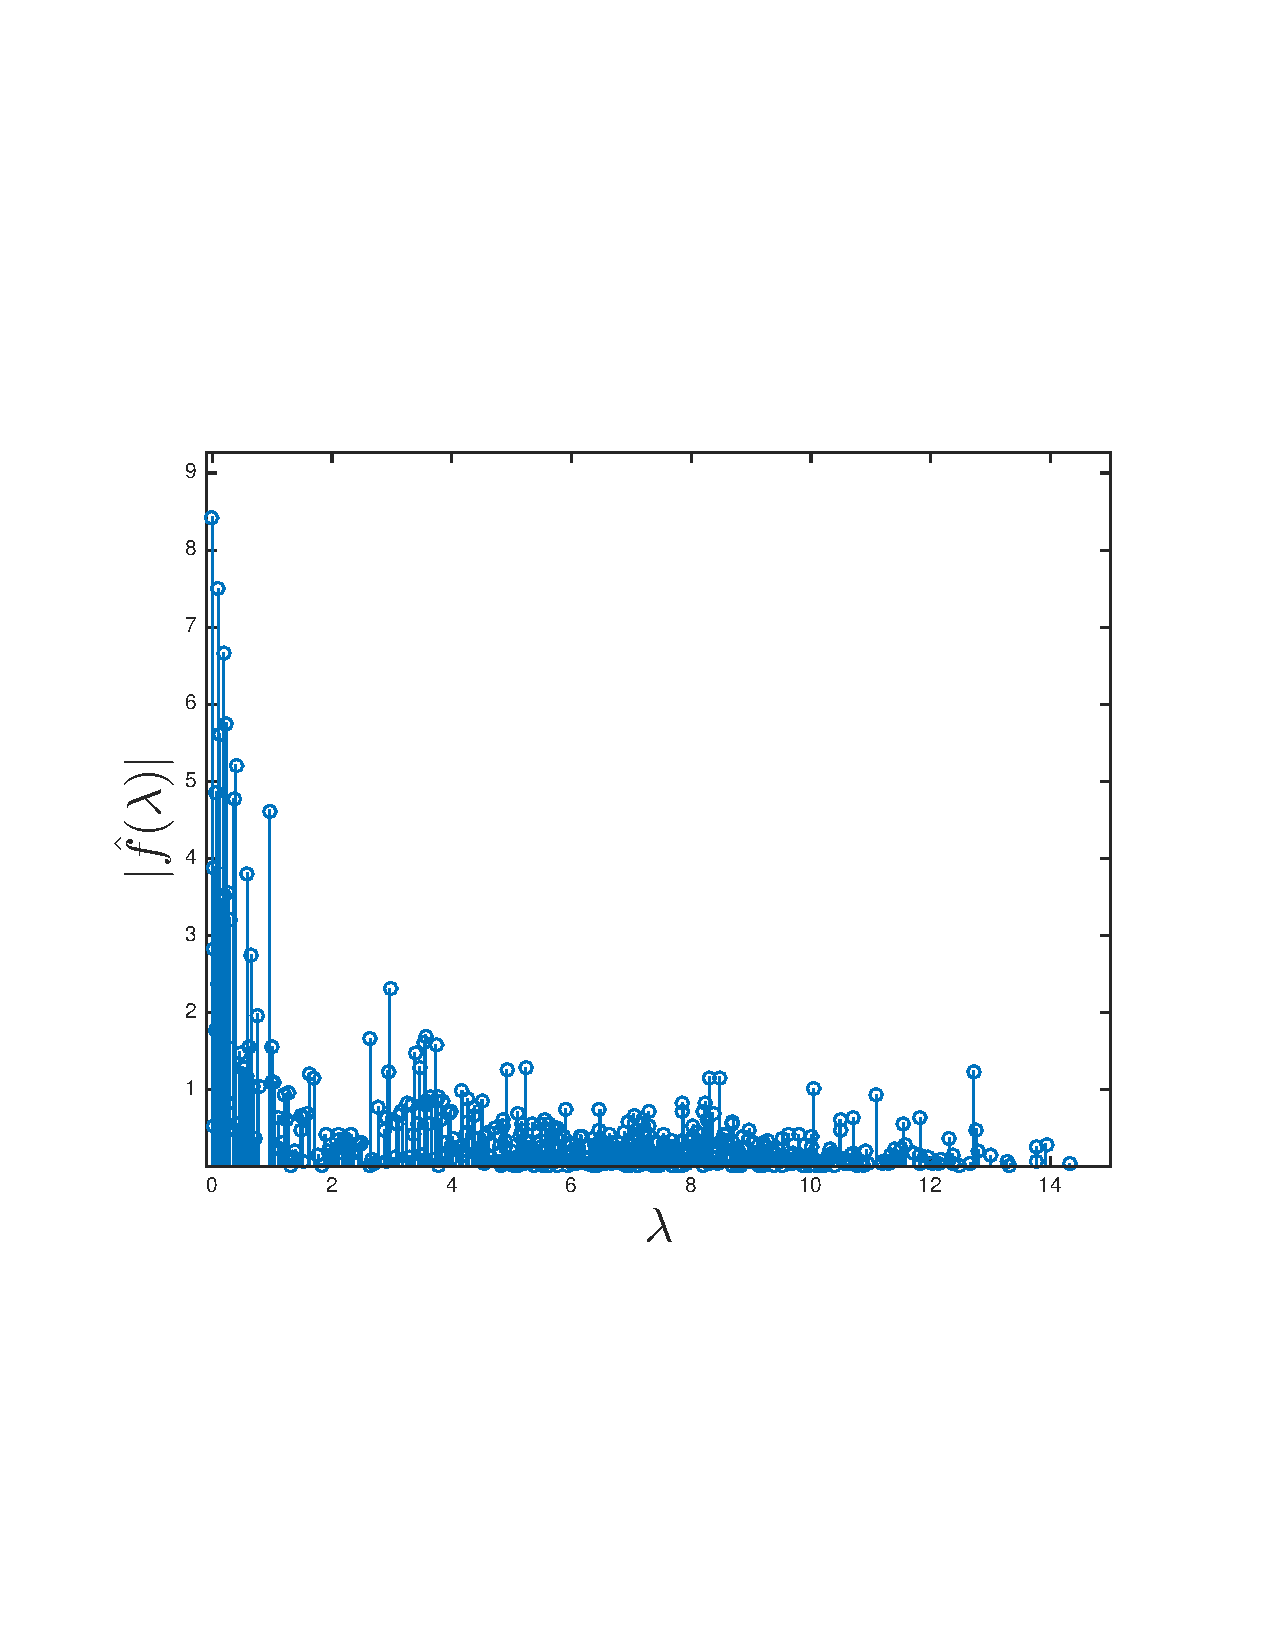
\includegraphics[width=.9\linewidth]{fig_comp_sig_hat}~}
\centerline{\small{(b)}}
\end{minipage} \\
\vspace{.07in}
\begin{minipage}[m]{0.48\linewidth}
\centerline{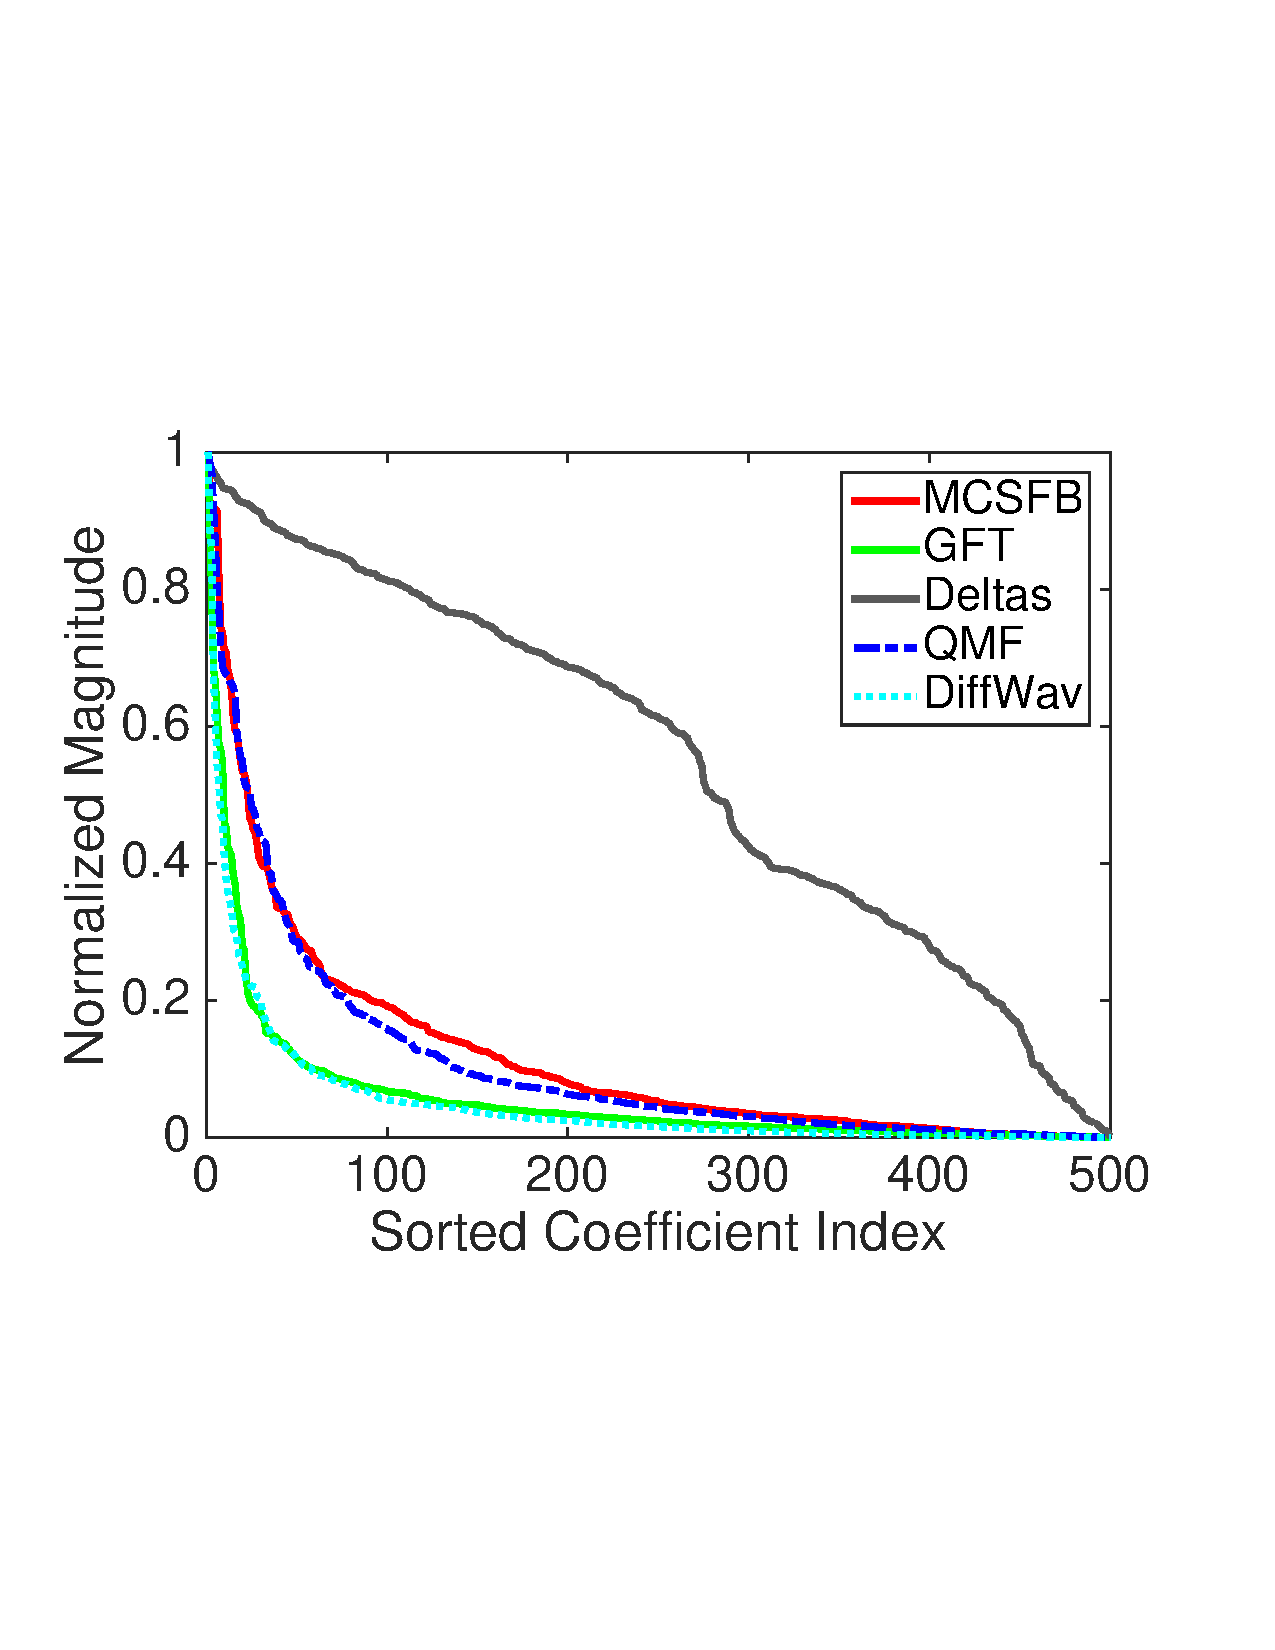
\includegraphics[width=.96\linewidth]{fig_comp_coeff2}}
\centerline{\small{(c)}}
\end{minipage}
\begin{minipage}[m]{0.48\linewidth}
\centerline{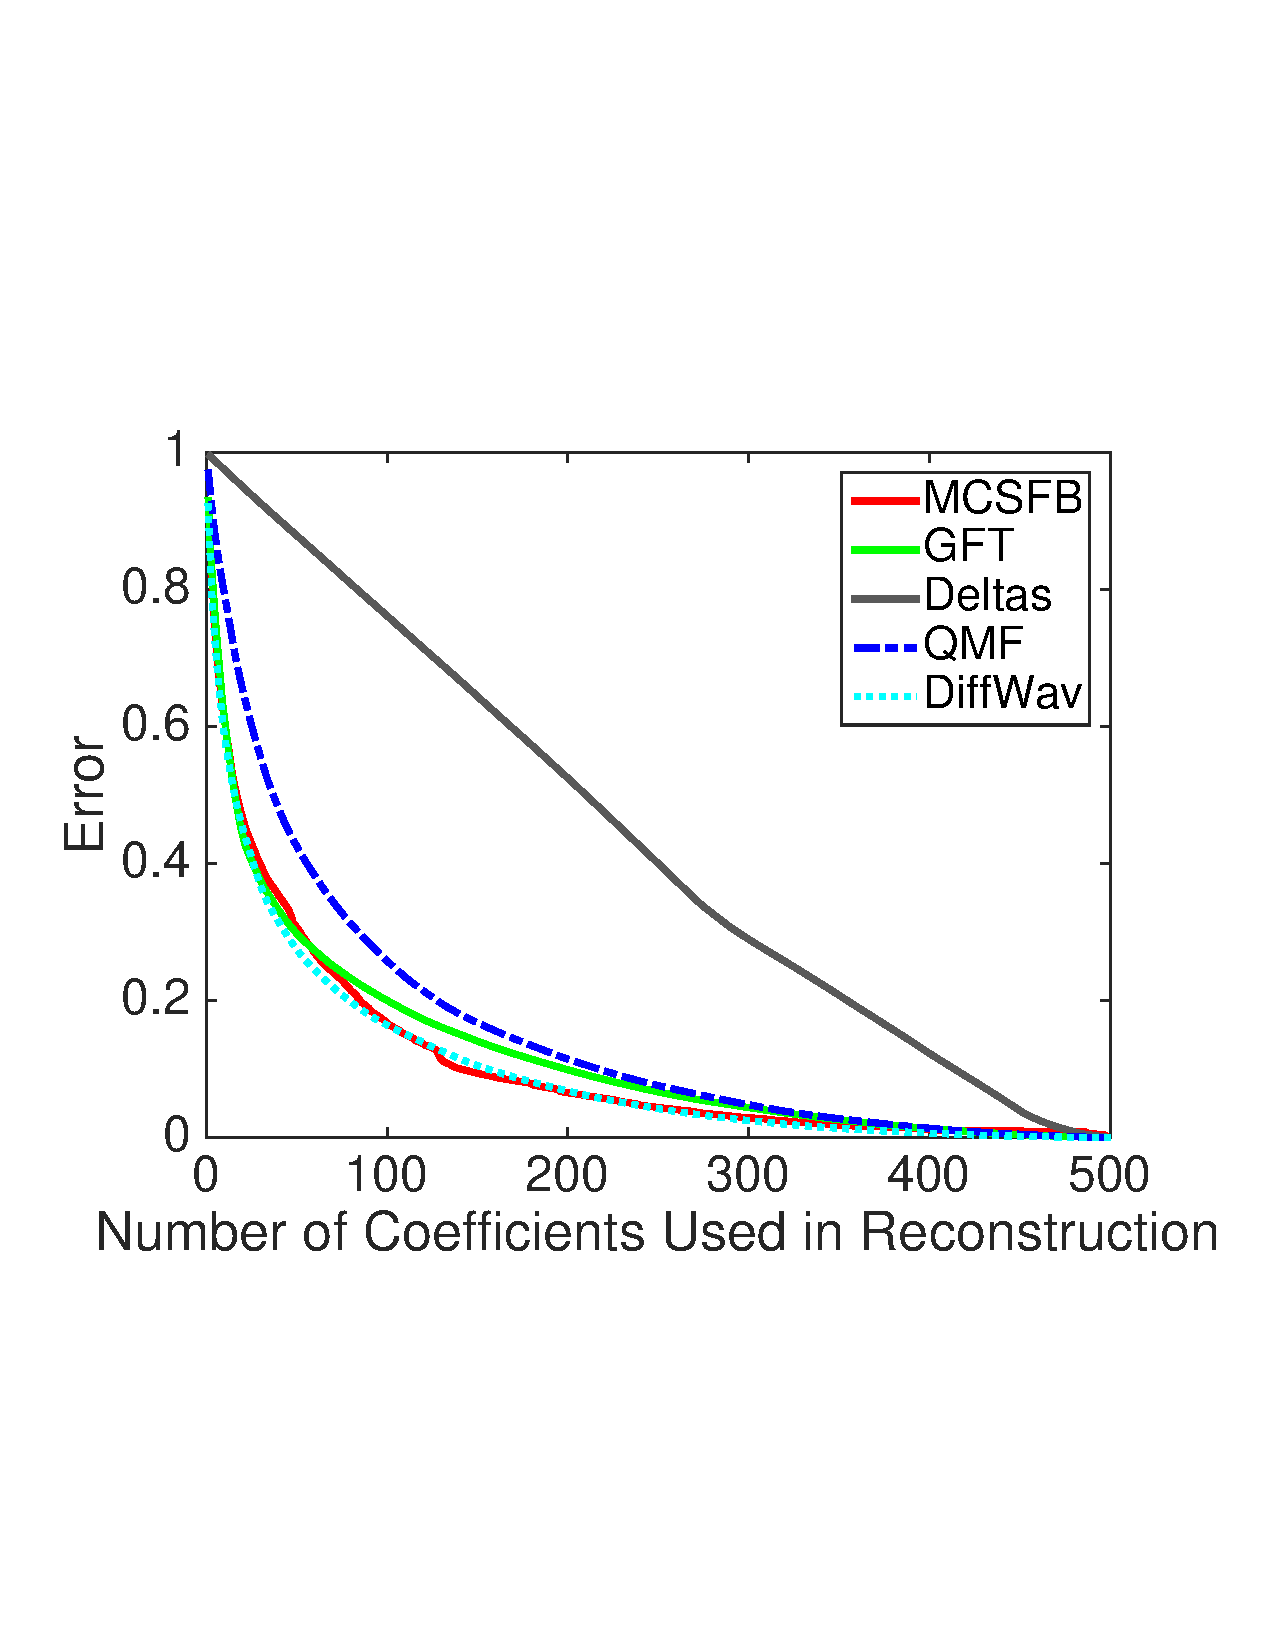
\includegraphics[width=.98\linewidth]{fig_comp_error}}
\centerline{\small{(d)}}
\end{minipage}
\caption{Compression example. (a)-(b) Piecewise-smooth signal from \cite[Fig. 11]{shuman_TSP_multiscale} in the vertex and graph spectral domains. (c) The normalized sorted magnitudes of the transform coefficients for the proposed $M$-channel critically sampled filter bank, the graph Fourier transform, the basis of Kronecker deltas, the quadrature mirror filterbank \cite{narang2012perfect}, and the diffusion wavelet transform \cite{coifman2006diffusion}. (d) The reconstruction errors  $\frac{\left|\left|f_{\mbox{reconstruction}}-f\right|\right|_2}{||f||_2}$, as a function of the sparsity threshold $T$ in \eqref{Eq:sparse_coding}.} \label{Fig:comp}
\end{figure}

{\color{blue}
\section{Filter Bank Design}
\begin{itemize}
\item Approximate filtering, and theory showing that the error (i) clusters around boundaries, and (ii) only matters where there are eigenvalues
\item Design to aim for spectral gaps
\end{itemize}

\section{Non-Uniform Sampling and Reconstruction}
\begin{itemize}
\item Estimating number of measurements for each band
\item Review of non-uniform random sampling literature
\item Reconstruction - emphasize change from only lowpass bands
\item {\color{red} Solving the reconstruction equation efficiently and robustly}
\end{itemize}

\section{Illustrative Examples II: Approximate Calculations}
\begin{itemize}
\item Make sure to have some very large examples and show computation times
\end{itemize}
}


\section{Ongoing Work}
\label{Sec:ongoing}
{\color{red} Eliminate once we've covered all of these issues elsewhere.}
We now briefly outline a number of extensions that we are currently investigating for the proposed transform.

\subsection{Computational approximations to improve scalability}
In the numerical examples in the previous sections, we have computed a full eigendecomposition of the graph Laplacian and subsequently used it for all three of the sampling, filtering, and interpolation operations; however, such an eigendecomposition does not scale well with the size of the graph as it requires ${\cal O}(N^3)$ operations with naive methods. We briefly mention a few potential computational approximations that would improve the scalability of the proposed filter bank.
\subsubsection{Sampling}

Reference \cite{anis2016efficient} has a nice review of the computational complexities of the various routines for identifying uniqueness sets.  The random sampling method proposed in \cite{PuyTGV15} does not require the full eigendecomposition of the graph Laplacian and therefore scales significantly better with the size of the graph.
We are currently examining whether there is a way to extend the approach of \cite{PuyTGV15} to non-uniformly randomly sample in a manner that leads with high probability to uniqueness sets for higher bands of the graph Laplacian spectrum.
 
\subsubsection{Filtering}\label{Se:filtering}
One possibility for efficiently designing the filter bank without full knowledge of the spectrum is to use the tight warped filter bank design of \cite{shuman2013spectrum}. These can either be adapted to the width of the spectrum using only an estimate of the maximum eigenvalue, or to an approximation of the eigenvalue distribution based on the spectrum slicing method of \cite[Section 3.3]{parlett}. In either case, the filters can then be applied using the polynomial approximation method discussed in \cite{hammond2011wavelets,shuman_DCOSS_2011}. An advantage of the approximation is that the value of the filtered signal at a given vertex is a weighted average of the signal values in a neighborhood around that vertex \cite{shuman2013emerging}. However, the interpolation step needs to be adjusted accordingly. 

\subsubsection{Interpolation}
If $y_{\V_m}$ are the analysis coefficients of the $m^{th}$ branch, the standard least squares reconstruction is to solve $x_m^*=\argmin_{x \in \R^{k_m}} ||\mathbf{U}_{{\cal R}_m}x - y_{\V_m} ||_2$, and let $f_{m,{rec}}(\V_m)=y_{\V_m}$ and $f_{m,{rec}}(\V_m^c)=\mathbf{U}_{\V_m^c,{\cal R}_m}x_m^*$; however, this requires a full eigendcomposition of $\L$ to get $\mathbf{U}$. Our ongoing work includes developing an efficient optimization algorithm that directly uses a function of $\L$ rather than $\mathbf{U}$ to stably reconstruct signals supported on a specific spectral band from its samples. 

\subsection{Reconstruction robustness to noisy or thresholded filter bank coefficients} \label{Se:noisy_ext}
For any partition into uniqueness sets, the proposed transform perfectly recovers the signal from the analysis coefficients. However, the choice of the downsampling patterns and interpolation method can dramatically affect the stability of the reconstruction if the analysis coefficients are corrupted by noise or are only partially available, or approximate filters are used to speed up the transform (see, e.g., \cite[Section III.B]{anis2016efficient} for more on reconstruction stability). Thus, we plan to investigate the role of the initial choice of the $\gamma_i$'s in Algorithm \ref{Al:uniqueness} in improving the stability of the reconstruction.

\subsection{Iterated filter bank} 
As with the classical wavelet construction, it is possible to iterate the filter bank on the output from the lowpass channel.
This could be beneficial, for example, in the case that we want to visualize the graph signal at different resolutions on  a sequence of coarser and coarser graphs. An interesting question is how iterating the filter bank with fewer channels at each step compares to a single filter bank with more channels and each filter supported on a smaller region of the spectrum.

\subsection{Signals that are sparsely represented by the MCSFB transform}
We  plan to more formally characterize the relationships between the decay of the analysis coefficients under the proposed transform and different properties of graph signals, as well as the underlying graph structure.
Globally smooth signals trivially lead to sparse analysis coefficients because the coefficients are only nonzero for first set of vertices in the partition. The same line of reasoning applies more generally to signals that are sparse in the graph spectral domain. More interesting is a theory for the coefficient decay for piecewise-smooth graph signals such as the ones shown in Fig. \ref{Fig:bunny_signal}(a) and Fig. \ref{Fig:comp}(a).

\balance
\bibliographystyle{IEEEtran}
{\small \bibliography{mcsfb_refs}}


\end{document}
